\documentclass[12pt]{article}



\usepackage{multicol}
\usepackage{graphicx} % rysunki
\usepackage[dvipsnames]{xcolor}
\usepackage{amssymb} % dla formu

\usepackage{amsmath}
\usepackage{bm}

\usepackage[utf8]{inputenc} %polskie czcionki
\usepackage[OT4]{polski} %polskie nazwy sekcji itp.

\usepackage{wasysym}

\usepackage{qtree}
\usepackage{epstopdf}

\usepackage{url}
%\date{} % delete this line to display the current date

\newtheorem{definicja}{Definicja}
\newtheorem{fakt}{Fakt}
\newtheorem{fact}{Fakt}
\newtheorem{ass}{Założenie}
\newtheorem{rul}{Reguła}

\newcommand {\KRZ} {\ensuremath{\mathbb{KRZ}}}
\newcommand {\PZWKRZ} {\ensuremath{\mathbb{PZW_{KRZ}}}}
\newcommand {\PZWWRP} {\ensuremath{\mathbb{PZW_{WRP}}}}
\newcommand {\WRP} {\ensuremath{\mathbb{WRP}}}
\newcommand {\KPN} {\ensuremath{\mathbb{KPN}}}
\newcommand {\IWRP} {\ensuremath{1 \mathbb{WRP}}}
\newcommand {\PZWIWRP} {\ensuremath{\mathbb{PZW}_{1 \mathbb{WRP}}}}
\newcommand {\AL} {\ensuremath{\mathbb{ALC}}}
\newcommand {\SROIQ} {\ensuremath{\mathcal{SROIQ}}}

\newcommand {\Type} {\ensuremath{\mathbb{TYPE}}}
\newcommand {\Rel} {\ensuremath{\mathbb{REL}}}



\begin{document}

\title{Podstawy logiki}
\author{KPI}


%%% BEGIN DOCUMENT

%\includeonlylecture{div}
\maketitle
\tableofcontents



\section{Klasyczny rachunek zdań}

\subsection{Rzut oka wstecz}

\subsection{\KRZ}
%
    \begin{itemize}
        \item dlaczego?
        \item co?
        \item jak?
        \item dla-czego-nie?
    \end{itemize}
%

\subsection{Skróty}
\begin{itemize}
\item \KRZ
\item \PZWKRZ
\item \WRP
\item \PZWWRP
\end{itemize}
%


%\subsection{Poprawność wnioskowania}
%
%\subsection{Typy poprawności wnioskowań}
%%
%\begin{itemize}
%\item Wnioskowanie jest \emph{poprawne materialnie} jeśli wszystkie jego przesłanki są prawdziwe.
%%
%\item Wnioskowanie jest \emph{poprawne formalnie} jeśli wniosek wynika z przesłanek, tzn. gdy nie może być tak, że przesłanki tego wnioskowania są prawdziwe, a wniosek fałszywy.
%%%
%%\item Wnioskowanie jest \emph{obarczone błędem petitio principii} jeśli uzasadnienie przynajmniej jednej z przesłanek (tego wnioskowania) wykorzystuje tę lub inną przesłankę tego samego wnioskowania.
%\end{itemize}
%%
%
%\subsection{Poprawność materialna - antyprzykład}
%%
%\begin{eqnarray*}
%\label{W2}
%& \textrm{\textbf{\alert{Tylko pojazdy silnikowe są wyposażone w silniki.}}} \nonumber \\
%& \textrm{Każdy (sprawny) motorower jest wyposażony w silnik}. \nonumber \\
%& \textrm{------------------------------------------------------------------------}\nonumber \\
%& \textrm{Każdy motorower jest pojazdem silnikowym.}
%\end{eqnarray*}
%%
%
%\subsection{Poprawność formalna - antyprzykład}
%%
%\begin{eqnarray*}
%\label{W3}
%& \textrm{Wszystkie pojazdy silnikowe są wyposażone w silniki.} \nonumber \\
%& \textrm{Każdy (sprawny) motorower jest wyposażony w silnik.} \nonumber \\
%& \textrm{\alert{\textbf{------------------------------------------------------------------------}}}\nonumber \\
%& \textrm{Każdy motorower jest pojazdem silnikowym.}
%\end{eqnarray*}
%%
%
%%\subsection{Błąd \emph{petitio principii} - przykład}
%%%
%%\begin{itemize}
%%\item[Jan] Bóg istnieje.
%%%
%%\item[Paweł] Dlaczego?
%%%
%%\item [Jan] Ponieważ tak mówi Biblia.
%%%
%%\item [Paweł] I co z tego?
%%%
%%\item [Jan] Biblia zawsze mówi prawdę.
%%%
%%\item [Paweł] Skąd ty to wiesz?
%%%
%%\item [Jan] Bo Bóg powiedział, że Biblia zawsze mówi prawdę.
%%%
%%\item [Paweł] Ale skąd w ogóle wiesz, że Bóg isnieje?
%%%
%%\item [Jan] Ponieważ tak mówi Biblia.
%%\end{itemize}
%%%
%
%%\subsection{Wnioskowania dedukcyjne}
%%\begin{figure}
%%\begin{center}
%%\includegraphics[scale=0.4]{wniosktypy.jpg}
%%\end{center}
%%\end{figure}
%%%
%
%\subsection{Wnioskowania dedukcyjne (2)}
%%
%\begin{definicja}Wnioskowanie jest \emph{dedukcyjne} jeżeli wniosek (tego wnioskowania) wynika \textbf{logicznie} z przesłanek.\end{definicja}
%%
%\begin{definicja} Zdanie $Z$ \emph{wynika logicznie} ze zdań $Z_1, Z_2, \dots, Z_n$ wtedy i tylko wtedy, gdy implikacja $$\text{Jeżeli~} Z_1 \text{~i~} Z_2 \text{~i \dots i~} Z_n \text{~, to~} Z$$ jest podstawieniem jakiegoś prawa logiki.\end{definicja}
%%
%\begin{definicja} Prawo logiki jest to prawdziwe zdanie zbudowane wyłącznie ze zmiennych, stałych logicznych i ewentualnie nawiasów.\end{definicja}
%%
%
%
%\subsection{Prawo logiki - przykłady}
%\begin{itemize}
%%
%\item $p$ lub nieprawda, że $p$.
%%
%\begin{itemize}
%\item jeżeli Donald Tusk jest premierem a Lech Kaczyński jest prezydentem, to prawdą jest, że \textbf{Donald Tusk jest premierem lub nie jest premierem}
%%
%\item jeżeli Donald Tusk jest prezydentem a Lech Kaczyński jest premierem, to prawdą jest, że \textbf{Donald Tusk jest premierem lub nie jest premierem}
%%
%\item jeżeli Maria Curie-Skłodowska była kobietą, to prawdą jest, że \textbf{Donald Tusk jest premierem lub nie jest premierem}
%\end{itemize}
%%
%\item prawem logiki \alert{nie jest} ``2+2=4''.
%\end{itemize}
%%
%
%\subsection{Wynikanie logiczne - przykłady}
%%
%\begin{itemize}
%\item <2-> przykłady:
 %\begin{itemize}
 %\item <3-5> Ze zdania:
    %\begin{itemize}
    %\item <3-5> Nieprawda, że Jan jest bogaty i uczciwy.
    %\end{itemize}
 %\item <4-5> wynika logicznie zdanie
    %\begin{itemize}
    %\item <4-5> Jan nie jest bogaty lub Jan nie jest uczciwy.
    %\end{itemize}
 %\end{itemize}
 %\begin{itemize}
 %\item <6-> Ze zdania:
    %\begin{itemize}
    %\item <6-> Jan ma więcej helikopterów niż Tadeusz.
    %\end{itemize}
 %\item <7-> \alert <8> {nie} wynika \textbf<8>{logicznie} zdanie:
    %\begin{itemize}
    %\item <7-> Tadeusz ma mniej helikopterów niż Jan.
    %\end{itemize}
 %\end{itemize}
%\end{itemize}
%%
%
%\subsection{Sprawdzanie poprawności formalnej wnioskowania  - przykład}
%<1>{\begin{eqnarray*}
%&\textrm{Jeżeli ten drut jest z miedzi, to jest dobrym przewodnikiem prądu.}\nonumber \\
%&\textrm{Ten drut jest dobrym przewodnikiem prądu.}\nonumber \\
%&\textrm{----------------------------------------------------------------------------------------}\nonumber \\
%&\textrm{Ten drut jest z miedzi.}
%\end{eqnarray*}}
%
%<2>{\begin{eqnarray*}
%&\textrm{Jeżeli~} \underbrace{\textrm{ten drut jest z miedzi}}_{p}, \textrm{~to~} \underbrace{\textrm{jest dobrym przewodnikiem prądu}}_{q}\nonumber \\
%&\underbrace{\textrm{Ten drut jest dobrym przewodnikiem prądu.}}_{q}\nonumber \\
%&\textrm{------------------------------------------------------------------------------}\nonumber \\
%&\underbrace{\textrm{Ten drut jest z miedzi.}}_{p}
%\end{eqnarray*}}
%
%<3-5>{\begin{eqnarray*}
%&\textrm{Jeżeli~} p, \textrm{~to~} q \nonumber \\
%& q \nonumber \\
%&\textrm{------------------------------------------------------------------------------}\nonumber \\
%&p
%\end{eqnarray*}}
%
%<4>{\begin{eqnarray*}
%(\textrm{Jeżeli~} p, \textrm{~to~} q) \textrm{~i~} q, \textrm{~to~} p.
%\end{eqnarray*}}
%
%<5>{\begin{eqnarray*}
%(p \to q) \land q \to p.
%\end{eqnarray*}}
%%
%
%\subsection{Sprawdzanie poprawności formalnej wnioskowania (2)}
%%
%\textbf{Ponieważ}
%$$(p \to q) \land q \to p.$$
%\alert{nie} jest prawem logiki,  \\ \textbf{więc} wnioskowanie 
%%
%\begin{eqnarray}\label{W4}
%&\textrm{Jeżeli ten drut jest z miedzi, to jest on dobrym przewodnikiem prądu.}\nonumber \\
%&\textrm{Ten drut jest dobrym przewodnikiem prądu.}\nonumber \\
%&\textrm{------------------------------------------------------------------------------------------}\nonumber \\
%&\textrm{Ten drut jest z miedzi.}
%\end{eqnarray}
%\alert{nie} jest dedukcyjne.
%%
%
%\subsection{Schematy wnioskowań}
%\begin{itemize}
%\item <1-> \emph{Formalny schemat wnioskowania} jest to układ form zdaniowych zbudowanych wyłącznie za pomocą stałych logicznych i zmiennych (ewentualnie nawiasów), takich, że są one (tzn. te formy) schematami przesłanek i wniosku tego wnioskowania.
%\begin{eqnarray}
%\label{schemat W1}
% <2-> {p \to q \nonumber \\
%\textrm{---------} \nonumber \\
%q \to p \nonumber \\}
%\end{eqnarray}
% <3> {\begin{eqnarray}
%\label{W5}
%& \textrm{Jeżeli dziś jest poniedziałek, to jutro jest wtorek.}\nonumber \\
%& \textrm{-------------------------------------------------------------------}\nonumber \\
%& \textrm{Jeżeli jutro jest wtorek, to dziś jest poniedziałek.}
%\end{eqnarray}}
% <4>{\begin{eqnarray}
%\label{W6}
%&\textrm{Jeżeli J. Kaczyński jest starym kawalerem, to jest on mężczyzną.}\nonumber \\
%&\textrm{-----------------------------------------------------------------------------------------}\nonumber \\
%&\textrm{Jeżeli J. Kaczyński jest mężczyzną, to jest starym kawalerem.}\nonumber \\
%&
%\end{eqnarray}}
%
%\end{itemize}
%%
%
%\subsection{Schematy wnioskowań (2)}
%\begin{itemize}
%\item Schematy wnioskowań dedukcyjnych są niezawodnymi sposobami komfortowego zdobywania wiedzy, tzn.  zawsze od prawdziwych przesłanek prowadzą do prawdziwego wniosku.
%%
%\begin{eqnarray*}
% <2-> {p \to q \nonumber \\
%\textrm{---------} \nonumber \\
%q \to p \nonumber \\}
%\end{eqnarray*}
%%
%\item \ref{schemat W1} nie jest schematem niezawodnym, tzn. czasami od prawdziwych przesłanek prowadzi do wniosku prawdziwego, a czasami od prawdziwych przesłanek prowadzi do fałszywego wniosku.
%\end{itemize}
%%
%
%\subsection{Entymematy}
%%
%\begin{itemize}
%\item Pozór poprawności wnioskowania 4 bierze się stąd, że jest ono entymematem.
%%
%\begin{definicja}
%Entymemat jest wnioskowaniem dedukcyjnym, w którym jedną z przesłanek przemilczano, najczęściej z powodu jej oczywistości.
%\end{definicja}
%%
%\item W wnioskowaniu 4 przemilczaną przesłanką jest zdanie ``Dziś jest poniedziałek \emph{wtedy i tylko wtedy, gdy} jutro jest wtorek''.
%\end{itemize}
%%
%
%\subsection{Sprawdzanie poprawności formalnej wnioskowań}
%\begin{figure}
%\begin{center}
%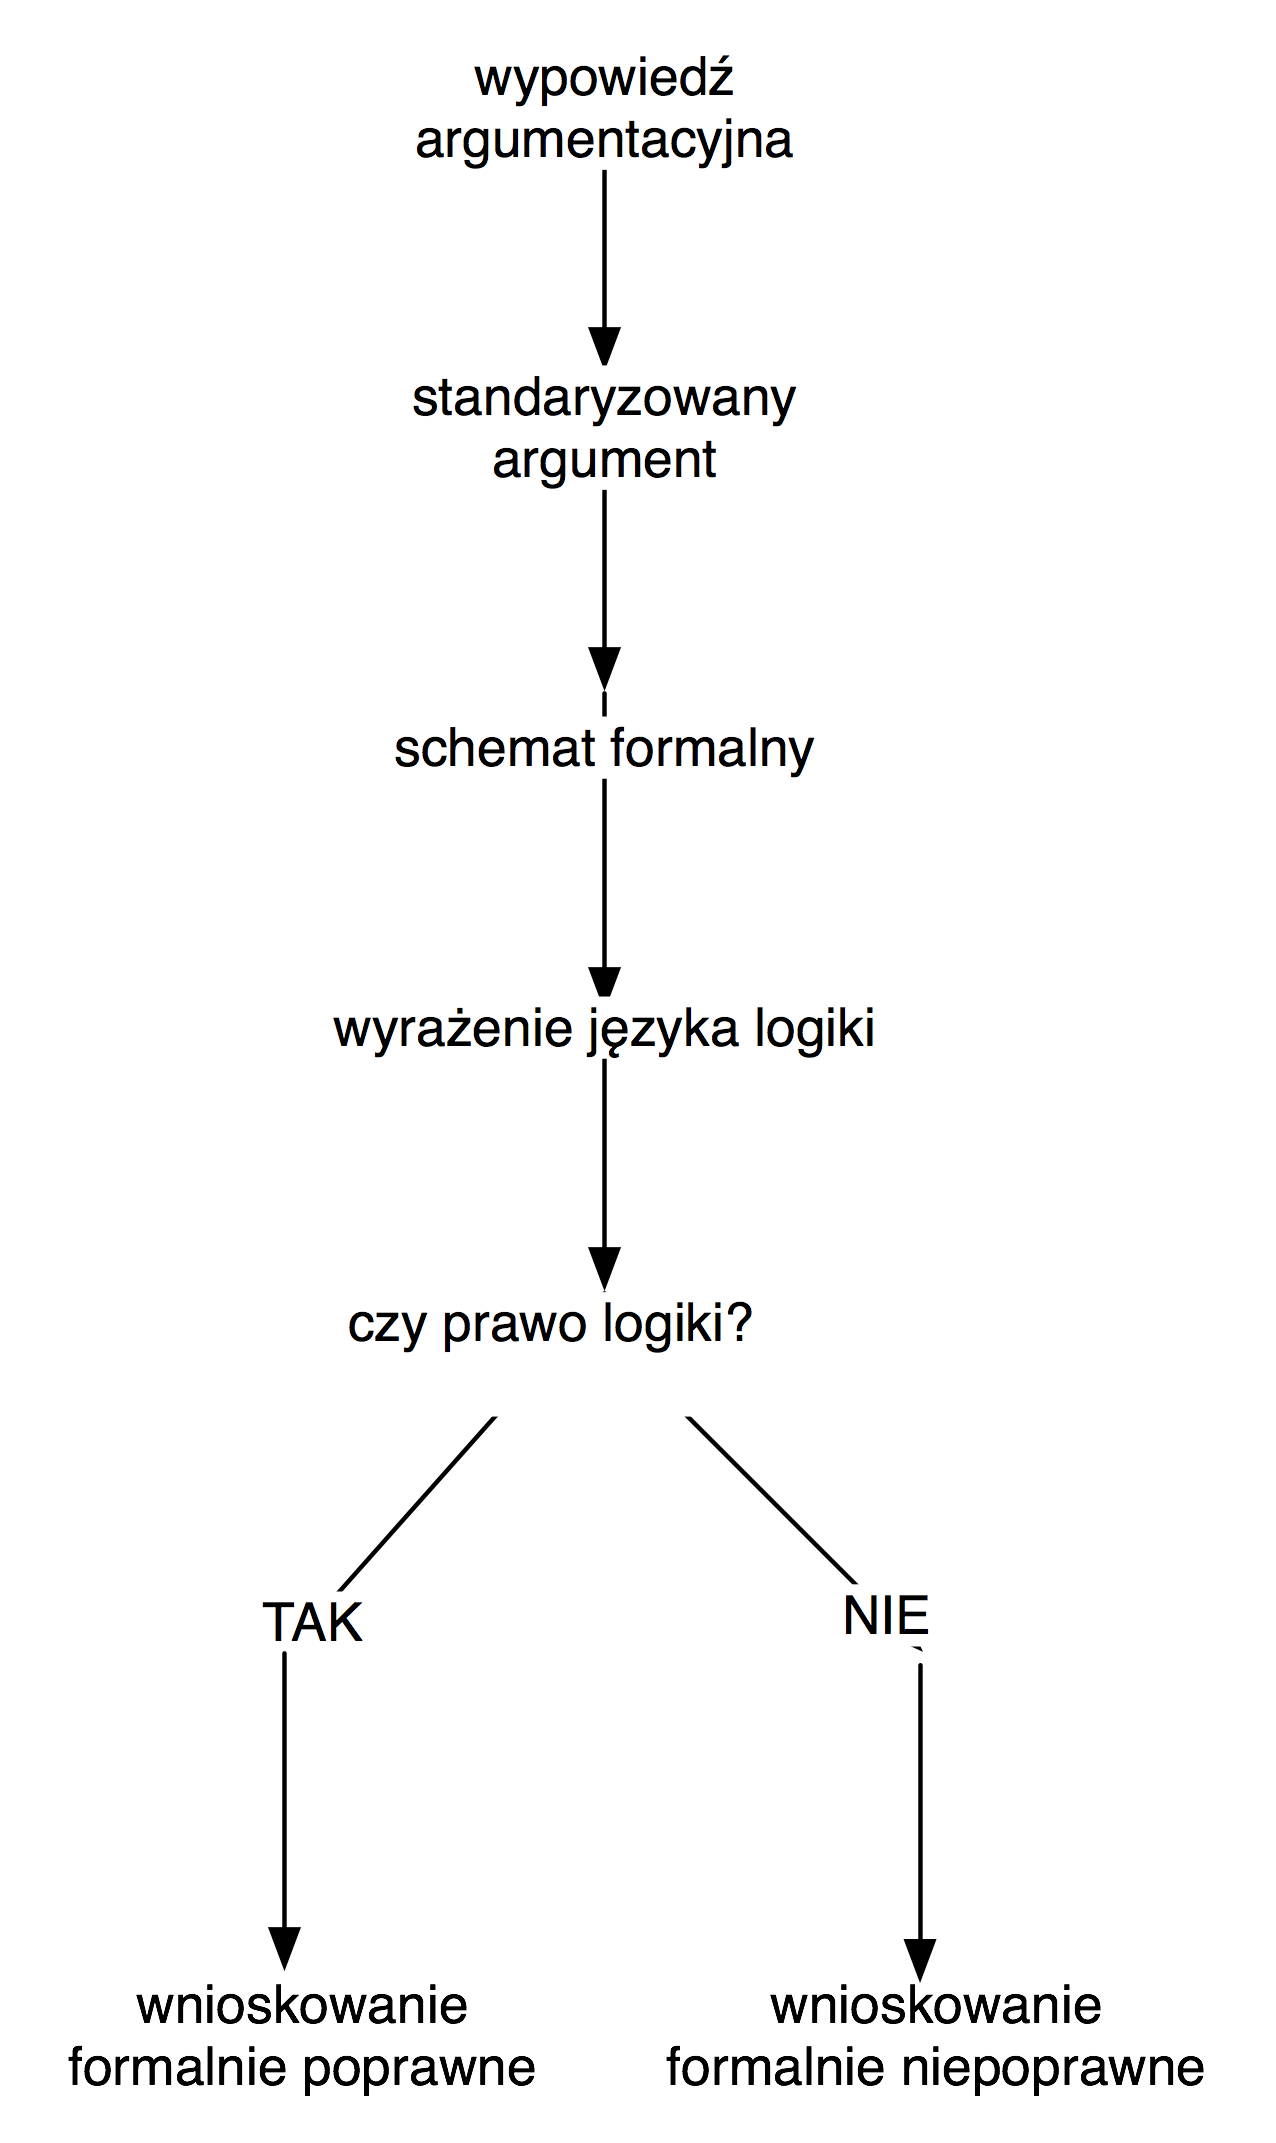
\includegraphics[scale=0.4]{check.jpg}
%\caption{Jak sprawdzać wnioskowania?}
%\end{center}
%\end{figure}
%%

\subsection{\PZWKRZ\ w notacji BNF}
%
\begin{equation}
\phi ~~::=~~ p ~|~ \neg \phi ~|~ \phi \land \phi ~|~ \phi \lor \phi ~|~ \phi \to \phi ~|~ \phi \equiv \phi
\end{equation}
%

\subsection{\PZWKRZ\ w notacji BNF (2)}
%
\begin{eqnarray}
<zero\_digit> :: = "0" \\ %
<nonzero\_digit> :: = "1" | "2" | "4" | "5" | "6" | "7" | "8" | "9" \\ %
<digit> :: = <zero\_digit> | <nonzero\_digit> \\ %
<index> :: = <digit> | <nonzero\_digit><index> \\ %
<atom> ::= "p"<index> \\  %
<\phi> ::= <atom> | \nonumber  \\
"(" "\neg"  <\phi> ")" | \nonumber \\
"(" <\phi> "\land" <\phi> ")" | \nonumber \\
"(" <\phi> "\lor" <\phi> ")" | \nonumber  \\
"(" <\phi> "\to" <\phi> ")" | \nonumber  \\
"(" <\phi> "\equiv" <\phi> ")"
\end{eqnarray}
%


\subsection{Metoda tablic analitycznych}

\subsection{Co każdy student chciałby wiedzieć o metodzie tablic analitycznych, ale wstydzi się zapytać}
%
\begin{itemize}
\item Praw \KRZ ~szukamy poprzez konstrukcję tablic analitycznych.\\
%
\item Metoda tablic jest zmodyfikowaną wersją skróconej metody zero-jedynkowej.\\
%
\item Tablica analityczna  jest binarnym drzewem znakowanym wyrażeniami \PZWKRZ.
\end{itemize}
%

\subsection{Metody \KRZ~ - porównanie}
% \begin{columns}[t]
% \begin{column}{4cm}
% \textbf{Metoda założeniowa} \\ \textcolor[rgb]{1.00,0.00,0.00}{trzeba myśleć} \\ \textcolor[rgb]{0.00,1.00,0.00}{nadaje się do} \WRP \\
% \end{column}
% \begin{column}{4cm}
% \textbf{Metoda 01-owa} \\ \textcolor[rgb]{0.00,1.00,0.00}{nie trzeba myśleć} \\ \textcolor[rgb]{0.98,0.00,0.00}{\emph{nie} nadaje się} do \WRP
% \end{column}
% \begin{column}{4cm}
% \textbf{Metoda tablic} \\ \textcolor[rgb]{0.00,1.00,0.00}{nie trzeba myśleć}  \\ \textcolor[rgb]{0.00,1.00,0.00}{nadaje się do} \WRP
% \end{column}
% \end{columns}
%


\subsection{Drzewa i drzewa}
%
\begin{center}
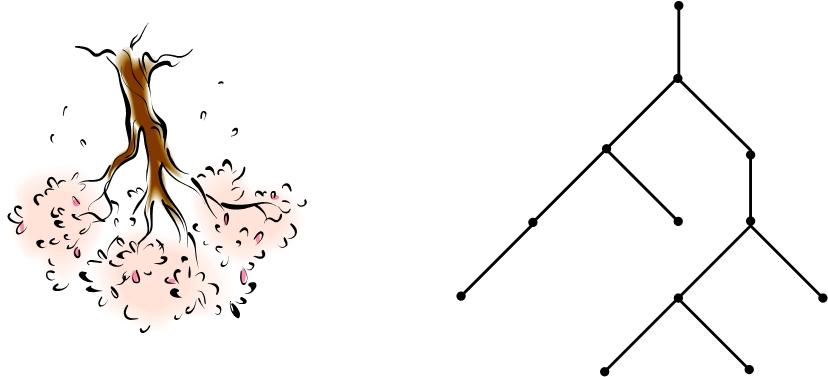
\includegraphics[width=6 cm]{../pliki_wlasne/drzewo0.jpg}
\end{center}
%


\subsection{Drzewa - korzenie i liście}
\begin{center}
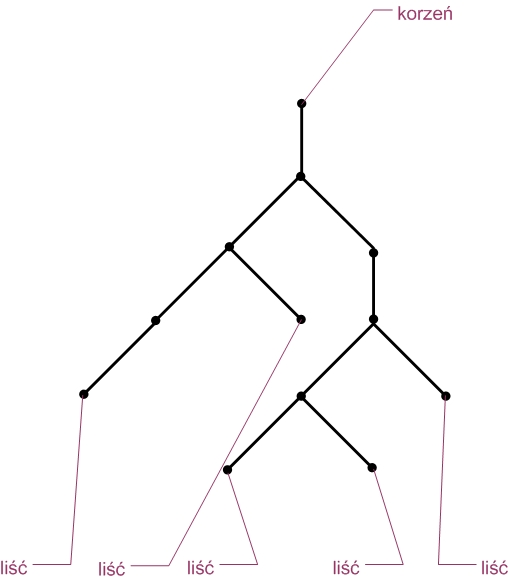
\includegraphics[width=6 cm]{../pliki_wlasne/drzewo1.jpg}
\end{center}
%

\subsection{Drzewa - gałęzie, korzenie i liście}
\begin{center}
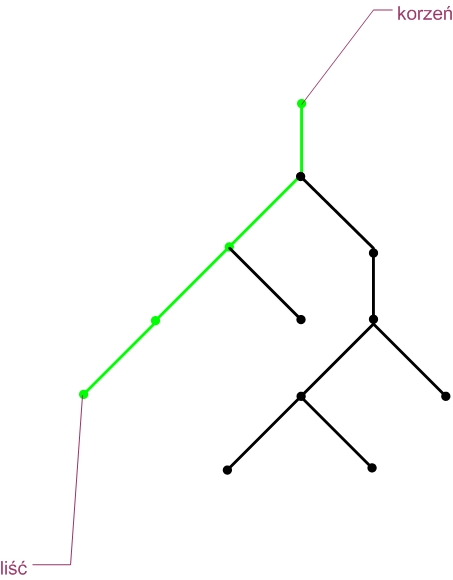
\includegraphics[width=6 cm]{../pliki_wlasne/drzewo2.jpg}
\end{center}
%

\begin{center}
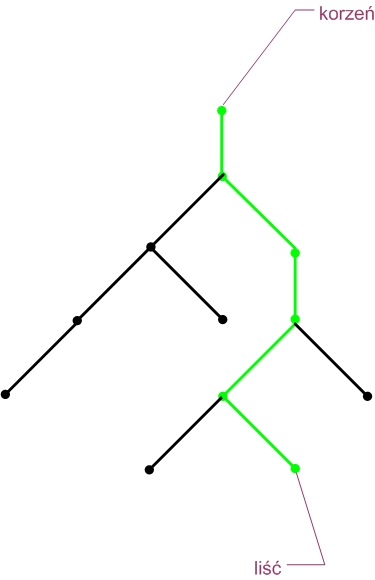
\includegraphics[width=5 cm]{../pliki_wlasne/drzewo3.jpg}
\end{center}
%

\begin{center}
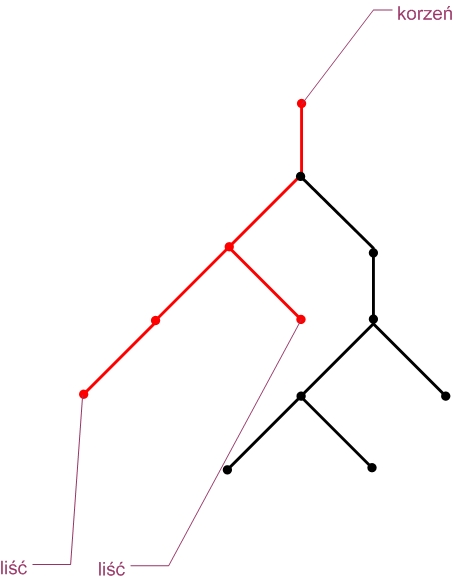
\includegraphics[width=6 cm]{../pliki_wlasne/drzewo4.jpg}
\end{center}
%

\subsection{Drzewa znakowane}
\begin{center}
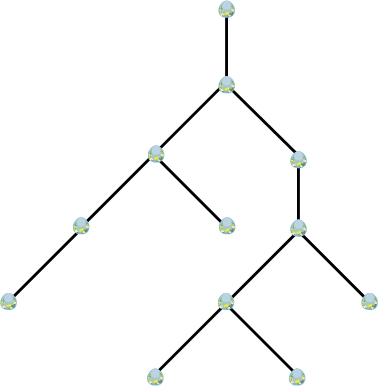
\includegraphics[width=6 cm]{../pliki_wlasne/drzewo5.jpg}
\end{center}
%

\begin{center}
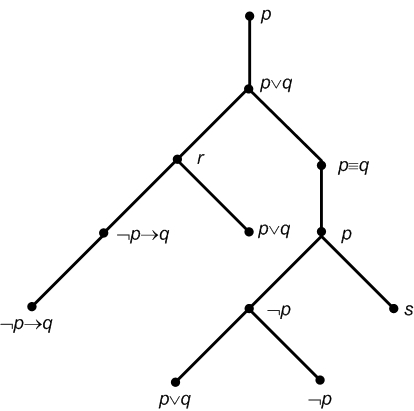
\includegraphics[width=7 cm]{../pliki_wlasne/drzewo6.jpg}
\end{center}
%

\subsection{Drzewa - nad/pod i obok}
\begin{center}
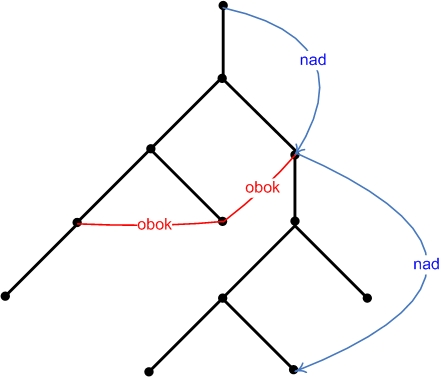
\includegraphics[width=7 cm]{../pliki_wlasne/drzewo7.jpg}
\end{center}
%

\subsection{Drzewa i poddrzewa}
\begin{center}
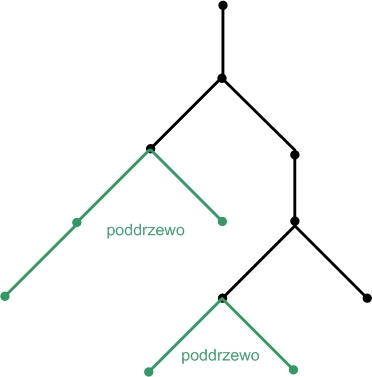
\includegraphics[width=7 cm]{../pliki_wlasne/drzewo8.jpg}
\end{center}
%

\begin{center}
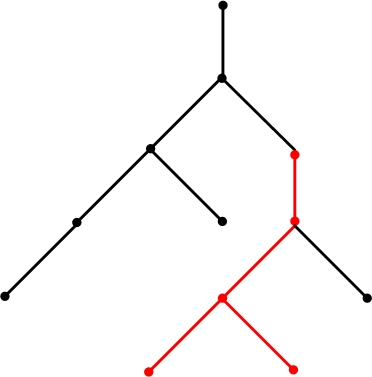
\includegraphics[width=7 cm]{../pliki_wlasne/drzewo9.jpg}
\end{center}
%

\subsection{Tablice analityczne -- skąd je brać?}
%
\begin{itemize}
\item Tablice analityczne składają się z atomowych tablic analitycznych.
%
\item Tworzenie tablic analitycznych polega na dodawaniu tablic atomowych do istniejącej tablicy.
%
\item W \KRZ~ mamy jedenaście tablic atomowych:
%
\begin{itemize}
\item \label{TA1} $\mathbb{T}$:~$p$
%
\item \label{TA2} $\mathbb{TN}$:~$\neg p$
%
\item \label{TA3} $\mathbb{TON}$: \Tree [.{$\neg \neg \phi$} $\phi$ ]
\end{itemize}
\end{itemize}
%

\begin{itemize}
\item \label{TA4} $\mathbb{TOK}$: \Tree [.{$\phi \land \psi$} [.$\phi$ [.$\psi$ ] ] ]
%
\item \label{TA5} $\mathbb{TOA}$: \Tree [.{$\phi \lor \psi$} $\phi$ $\psi$ ]
%
\item \label{TA6} $\mathbb{TOC}$: \Tree [.{$\phi \to \psi$} {$\neg \phi$} $\psi$ ]
\end{itemize}
%

\begin{itemize}
\item \label{TA7} $\mathbb{TOE}$: \Tree [.{$\phi \equiv \psi$} [.$\phi$ [.$\psi$ ] ] [.$\neg \phi$ [.$\neg \psi$ ] ] ]
%
\item \label{TA8} $\mathbb{TONK}$: \Tree [.{$\neg(\phi \land \psi)$} {$\neg \phi$} {$\neg \psi$} ]
%
\item \label{TA9} $\mathbb{TONA}$: \Tree [.{$\neg(\phi \lor \psi)$} [.{$\neg \phi$} [.{$\neg \psi$} ] ] ]
\end{itemize}
%

\begin{itemize}
\item \label{TA10} $\mathbb{TONC}$: \Tree [.{$\neg (\phi \to \psi)$} [.$\phi$ [.{$\neg \psi$} ] ] ]
%
\item \label{TA11} $\mathbb{TONE}$: \Tree [.{$\neg (\phi \equiv \psi)$} [.$\phi$ [.{$\neg \psi$} ] ] [.{$\neg \phi$} [.{$ \psi$} ] ] ]
\end{itemize}
%

\subsection{Zredukowane tablice analityczne}
\begin{itemize}
\item Tablice analityczne konstruujemy tak długo, aż uzyskamy zredukowaną ich postać.
%
\item Jeżeli $\phi$ jest wyrażeniem \KRZ, tj. gdy należy do \PZWKRZ, to symbol $T_{\phi}$ oznacza drzewo atomowe, które ma w korzeniu $\phi$.
%
\begin{definicja} Niech $T$ będzie tablicą analityczną.
\begin{enumerate}
\item wyrażenie $\phi$ jest \emph{zredukowane} w $T$ jeżeli drzewo $T'_{\phi}$ jest poddrzewem $T$.
\item Tablica analityczna $T$ jest \emph{zredukowana} jeżeli wszystkie wyrażenia z $T$ są zredukowane w $T$.
\end{enumerate}
\end{definicja}
\end{itemize}
%

\subsection{Zamknięte i otwarte tablice analityczne}
Po uzyskaniu tablicy zredukowanej sprawdzamy, czy uzyskana tablica jest otwarta, czy zamknięta.
%
\begin{definicja}
Tablice analityczna jest \emph{zamknięta}, jeżeli każda jej gałąź zawiera dwa wyrażenia sprzeczne: $\phi$, $\neg \phi$. \\
Tablice analityczna jest \emph{otwarta}, jeżeli nie jest zamknięta.
\end{definicja}
%
\begin{fact}
Wyrażenie $\phi \in \PZWKRZ$ jest prawem logiki wtedy i tylko wtedy, gdy istnieje zamknięta tablica analityczna dla $\neg \phi$.
\end{fact}
%

\subsection{Metoda tablic analitycznych - krok po kroku}
Czy $\phi \in \PZWKRZ$ jest prawem logiki?
%
\begin{enumerate}
\item Wstaw $\neg \phi$ jako korzeń tablicy analitycznej $T$!
%
\item Korzystając z atomowych tablic analitycznych zredukuj $T$!
%
\item Czy $T$ jest zamknięta?
%
\begin{itemize}
\item \textcolor[rgb]{0.00,1.00,0.00}{TAK} $\Longrightarrow$ $\phi$ \textcolor[rgb]{0.00,1.00,0.00}{jest} prawem logiki.
%
\item \textcolor[rgb]{1.00,0.00,0.00}{NIE} $\Longrightarrow$ $\phi$ \textcolor[rgb]{0.98,0.00,0.00}{nie jest} prawem logiki.
\end{itemize}
\end{enumerate}
%

\subsection{Metoda tablic analitycznych - przykłady}
<1> {Czy wyrażenie $(p \to q) \to p \lor q$ jest prawem logiki?\\}
<2> {\Tree [.{$\neg((p \to q) \to p \lor q)$} ]}
<3> {\Tree [.{$\neg((p \to q) \to p \lor q)$} [.{$p \to q$} [.{$\neg (p \lor q)$} ] ] ]}
<4> {\Tree [.{$\neg((p \to q) \to p \lor q)$} [.{$p \to q$} [.{$\neg (p \lor q)$} [.{$ \neg p$} {$\neg q$} ] ] ] ]\\}
<5> {\Tree [.{$\neg((p \to q) \to p \lor q)$} [.{$p \to q$} [.{$\neg (p \lor q)$} [.{$ \neg p$} [.{$\neg q$} {$\neg p$} $q$ ] ] ] ] ]\\}
%\Tree [.{$\neg((p \to q) \to p \lor q)$} [.{$p \to q$} [.{$\neg (p \lor q)$} [.{$ \neg p$} [.{$\neg q$} {$\neg p$} $q$ ] ] ] ] ]\\
%

\subsection{Metoda tablic analitycznych - przykłady (2)}
Ponieważ następująca gałąź w tej tablicy \emph{nie} zawiera wyrażeń \emph{sprzecznych}:\\
\Tree [.{$\neg((p \to q) \to p \lor q)$} [.{$p \to q$} [.{$\neg (p \lor q)$} [.{$ \neg p$} [.{$\neg q$} {$\neg p$} [. ] ] ] ] ] ]\\
%
zatem wyrażenie $(p \to q) \to p \lor q$ \emph{nie} jest prawem logiki, bo uzyskana tablica analityczna jest otwarta.\\
%

\subsection{Metoda tablic analitycznych - przykłady (3)}
<1> {Czy wyrażenie $q \to (p \to q)$ jest prawem logiki?\\}
<2>{\Tree [.{$\neg(q \to (p \to q))$} ] \\}
<3> {\Tree [.{$\neg(q \to (p \to q))$} [.$q$ {$\neg (p \to q)$}   ] ] \\}
<4> {\Tree [.{$\neg(q \to (p \to q))$} [.$q$ [.{$\neg (p \to q)$} [.$p$ {$\neg q$} ] ] ] ] \\}
<5> {Ponieważ jedyna gałąź w tej tablicy zawiera wyrażenia \emph{sprzeczne}: $q$, $\neg q$, zatem wyrażenie $q \to (p \to q)$ \emph{jest} prawem logiki.}
%

\subsection{Modele i kontrmodele}
\begin{itemize}
	\item model i kontrmodel formuły
	\item modele a drzewa
\end{itemize}
%

\subsection{Automatyzacja metody drzew/tablic}
\begin{itemize}
	\item \url{https://www.umsu.de/trees/}
\end{itemize}
%



\subsection{Metalogiczne własności \KRZ}

\subsection{Metalogiczne własności \KRZ}
    \begin{enumerate}
        \item \KRZ\ jest niesprzeczny
        \item \KRZ\ jest (zu)pełny
        \item \KRZ\ jest rozstrzygalny
    \end{enumerate}
%

\subsection{Tezy i tautologie w logice}
%
\begin{itemize}
    \item \emph{Teza} jest to wyrażenie zdaniowe, dla którego istnieje dowód ($\vdash \phi$).%
    \item \emph{Tautologia} jest to (zawsze) prawdziwe wyrażenie zdaniowe ($\vDash \phi$).
\end{itemize}
%

\subsection{Niesprzeczność teorii logicznej}%
\begin{itemize}
\item \emph{Teoria logiczna} jest to zbiór tez ("zamknięty" ze względu na dowody.)%
\item Teoria logiczna jest \emph{niesprzeczna} jeżeli wśród jej tez nie ma wyrażeń sprzecznych: $\phi$ i $\neg \phi$.
\end{itemize}
%

\subsection{Zdrowie i  pełność teorii logicznej}%
\begin{itemize}
    \item Teoria logiczna jest zdrowa (\emph{sound}), gdy każda jej teza jest tautologią.%
    \item Teoria logiczna jest pełna (\emph{complete}), gdy każda jej tautologia jest tezą.
\end{itemize}
%

\subsection{Rozstrzygalność teorii logicznej}%
\begin{itemize}
    \item Teoria logiczna jest \emph{rozstrzygalna}, gdy istnieje metoda, która w skończonej liczbie ściśle określonych kroków jest w stanie stwierdzić o każdym wyrażeniu, czy jest ono tezą tej teorii czy nie.%
    \item Teoria logiczna jest rozstrzygalna, gdy zbiór jej tez może zostać obliczony przez jakąś maszynę Turinga.
\end{itemize}
%

\section{Węższy rachunek predykatów}
\subsection{Motywacja}

\subsection{Poza \KRZ}
Pewne wnioskowania dedukcyjne są poza zasięgiem \KRZ:
%
\begin{itemize}
\item wnioskowania łatwe, np.:
%
\begin{eqnarray*}
%\label{W2}
& \textrm{Żaden gryzoń nie jest gadem.} \nonumber \\
& \textrm{------------------------------------------------------------------------}\nonumber \\
& \textrm{Nieprawda, że niektóre gady są gryzoniami.}
\end{eqnarray*}
%
\item wnioskowania trudne, np.:
%
\begin{eqnarray*}
& \textrm{Dłużnicy naszych dłużników są naszymi dłużnikami.}\nonumber \\
& \textrm{Każdy jest dłużnikiem swego każdego wierzyciela.}\nonumber \\
& \textrm{Każdy jest wierzycielem swego każdego dłużnika.}\nonumber \\
& \textrm{---------------------------------------------------------------------------------}\nonumber \\
& \textrm{Wierzyciele naszych wierzycieli są naszymi wierzycielami.}
\end{eqnarray*}
\end{itemize}
%

\subsection{Porównanie języków}
\begin{table}[p]
\begin{center}
{\scriptsize
\begin{tabular}{|c||c|c|c|}
\hline
\textbf{Wiedza} & \KRZ & \textbf{sylogistyka} & \WRP \\
\hline
Jan jest bogaty & $p$ & - & $A(\textrm{a})$ \\
\hline
Warszawa jest stolicą Polski & $p$ & - & $P(\textrm{a}, \textrm{b})$\\
\hline
Jan jest bogaty lub uczciwy & $p \lor q$ & - & $A(\textrm{a}) \lor B(\textrm{a})$\\
\hline
Anna lub Jan są bogaci & $p \lor q$ & - & $A(\textrm{a}) \lor A(\textrm{b})$\\
\hline
Każdy student jest uczciwy & $p$ & $S\textrm{a}P$ & $\forall x~(C(x) \to B(x))$ \\
\hline
Żaden student nie jest uczciwy & $p$ & $S\textrm{e}P$ & $\forall x~(C(x) \to \neg B(x))$ \\
\hline
Każdy student jest uczciwy lub odważny & $p$ & - & $\forall x~(C(x) \to B(x) \lor D(x))$ \\
\hline
Każdy syn Jana jest wrogiem Piotra & $p$ & - & $\forall x~(P(x,\textrm{a}) \to Q(x,\textrm{b}))$ \\
\hline
\end{tabular}
}
\caption{Wiedza w językach logiki}
\label{Comparison}

\end{center}

\end{table}
%

\subsection{Język \WRP}

\subsection{Predykaty}
predykaty:
%
\begin{itemize}
\item jednoargumentowe:
\begin{itemize}
\item \dots umiera,
\item \dots jest nieparzysta.
\end{itemize}
%
\item wieloargumentowe:
\begin{itemize}
\item $\dots < \dots$,
\item $\dots \in \dots$,
%
\item \dots kocha \dots,
%
\item \dots leży pomiędzy \dots a \dots.
\end{itemize}
\end{itemize}
%


\subsection{Alfabet \WRP}
%
\begin{definicja}
\label{alfabet (WRP)}
Alfabet \WRP~zawiera:
%
\begin{enumerate}
\item nieskończony zbiór zmiennych indywidualnych: $x, y, z, \dots, x_{1}, y_{1}, z_{1}, \dots, x_{2}, \dots$,
%
\item nieskończony zbiór stałych indywidualnych: $\textrm{a}, \textrm{b}, \textrm{c}, \dots, \textrm{a}_{1}, \textrm{b}_{1}, \textrm{c}_{1}, \dots, \textrm{a}_{2}, \dots$,
%
\item nieskończony zbiór predykatów:
\begin{itemize}
\item jednoargumentowych: $A, B, C, \dots, A_{1}, \dots$,
\item wieloargumentowych: $P, Q, R, \dots, P_{1}, \dots$,
\end{itemize}
%
\item zbiór funktorów prawdziwościowych: $\neg, \land, \lor, \to, \equiv$,
%
\item zbiór kwantyfikatorów: $\forall, \exists$,
%
\item nawiasy: (, ).
\end{enumerate}
\end{definicja}
%

\subsection{Język \WRP}
%
Sumę zbiorów:
\begin{enumerate}
\item zmiennych indywidualnych
\item stałych indywidualnych
%\item form nazwowych
\end{enumerate}
będziemy nazywać zbiorem \emph{wyrażeń nazwowych} \WRP.\\
%
Dowolny ciąg elementów alfabetu \WRP~jest \emph{napisem} (\WRP).
%

\subsection{Język \WRP (2)}
%
\begin{definicja}
\label{PZWWRP}
Zbiór poprawnie zbudowanych wyrażeń \WRP~(skrót: \PZWWRP) jest najmniejszym zbiorem napisów spełniającym poniższe warunki:
%
\begin{enumerate}
\item Jeżeli $\delta^{(n)}$ jest predykatem $n$-argumentowym $(n \geq 1)$, a $\alpha_{1}, \alpha_{2}, \dots, \alpha_{n}$ są wyrażeniami nazwowymi, to $\delta^{(n)}(\alpha_{1}, \alpha_{2}, \dots, \alpha_{n}) \in \PZWWRP$.% Wyrażenie $\delta^{(n)}(\alpha_{1}, \alpha_{2}, \dots, \alpha_{n})$ jest wyrażeniem atomicznym \WRP.%
\item Jeśli $\phi \in \PZWWRP$, to $\neg \phi \in \PZWWRP$.
%
\item Jeśli $\phi, \psi \in \PZWWRP$, to $(\phi \land \psi), (\phi \lor \psi), (\phi \to \psi), (\phi \equiv \psi) \in \PZWWRP$.
%
\item Jeżeli $\phi \in \PZWWRP$ i $\alpha$ jest zmienną indywidualną, to $\forall \alpha (\phi)$ i $\exists \alpha (\phi) \in \PZWWRP$.
\end{enumerate}
\end{definicja}
%

\subsection{Alfabet \WRP\ -- notacja BNF}
%
\begin{eqnarray}
<zero\_digit> :: = "0" \\ %
<nonzero\_digit> :: = "1" | "2" | "4" | "5" | "6" | "7" | "8" | "9" \\ %
<digit> :: = <zero\_digit> | <nonzero\_digit> \\ %
<index> :: = <digit> | <nonzero\_digit><index> \\ %
<const> ::= "a"<index> \\ %
<var> ::= "x"<index> \\ %
<\alpha> ::= <const> | <var> \\ %
<seq> ::= <\alpha> | <\alpha>","<seq> \\ %
<pred> ::= "P"<index>
\end{eqnarray}
%

\subsection{Język \WRP\ -- notacja BNF}
%
\begin{eqnarray}
<atom> ::= <pred>"("<seq>")" \\
%
<\phi> ::= <atom> | \nonumber  \\ 
"\forall"<var> \phi | \nonumber  \\
"\exists"<var> \phi | \nonumber  \\
"\neg" <\phi> | \nonumber  \\
<\phi> "\land" <\phi> | \nonumber \\
<\phi> "\lor" <\phi> | \nonumber  \\
<\phi> "\to" <\phi> | \nonumber  \\
<\phi> "\equiv" <\phi>
\end{eqnarray}
%

\subsection{O zmiennych i stałych - ponownie}
%
\begin{itemize}
\item zmienne:
\begin{itemize}
\item reprezentują wyrażenia/stałe
\item występują w językach:
\begin{itemize}
\item matematyki i nauk ścisłych
\item logiki
\item językach programowania
\end{itemize}
\item \emph{nie} występują w językach etnicznych
\begin{itemize}
\item coś, ktoś, gdzieś, itp.
\item Coś zjadło mój ser.
\end{itemize}
\end{itemize}
%
\item stałe:
\begin{itemize}
\item nic nie reprezentują
\item występują w każdym języku
\item występują w językach etnicznych
\begin{itemize}
\item Bruno zjadł mój ser.
\end{itemize}
\end{itemize}
\end{itemize}
%

\subsection{Notacja nawiasowa zredukowana w \WRP}
W ciągu symboli: kwantyfikator: $\forall$ lub $\exists$, $\neg, \land, \lor, \to, \equiv$, każdy symbol wiąże krócej (=silniej) niż symbole występujące po nim.
%

%\subsection{Notacja nawiasowa zredukowana w \WRP (2)}
%\begin{table}[p]
%\begin{center}
%\begin{tabular}{|c|c|}
%\hline
%\bf{Pełna notacja nawiasowa} & \bf{Zredukowana notacja nawiasowa}\\
%\hline
%$(\phi \land \psi) \lor \chi$ & $\phi \land \psi \lor \chi$ \\
%\hline
%$ \chi \lor (\phi \land \psi)$ & $\chi \lor \phi \land \psi$ \\
%\hline
%$(\phi \land \psi) \to \chi$ & $\phi \land \psi \to \chi$ \\
%\hline
%$ \chi \to (\phi \land \psi)$ & $\chi \to \phi \land \psi$ \\
%\hline
%$(\phi \land \psi) \equiv \chi$ & $\phi \land \psi \equiv \chi$ \\
%\hline
%$ \chi \equiv (\phi \land \psi)$ & $\chi \equiv \phi \land \psi$ \\
%\hline
%$(\phi \lor \psi) \to \chi$ & $\phi \lor \psi \to \chi$ \\
%\hline
%$ \chi \to (\phi \lor \psi)$ & $\chi \to \phi \lor \psi$ \\
%\hline
%$(\phi \lor \psi) \equiv \chi$ & $\phi \lor \psi \equiv \chi$ \\
%\hline
%$ \chi \equiv (\phi \lor \psi)$ & $\chi \equiv \phi \lor \psi$ \\
%\hline
%$(\phi \to \psi) \equiv \chi$ & $\phi \to \psi \equiv \chi$ \\
%\hline
%$ \chi \equiv (\phi \to \psi)$ & $\chi \equiv \phi \to \psi$ \\
%\hline
%\end{tabular}
%\caption{Redukcja nawiasów w wyrażeniach \KRZ}
%\label{RedukcjaPZWKRZ}
%\end{center}
%\end{table}
%%
%
%\subsection{Notacja nawiasowa zredukowana w \WRP\ (3)}
%\begin{table}[p]
%
%\begin{center}
%\begin{tabular}{|c|c|}
%\hline
%\bf{Pełna notacja nawiasowa} & \bf{Zredukowana notacja nawiasowa}\\
%\hline
%%$\forall \alpha (\neg \phi)$ & $\forall \alpha~ \neg \phi$ \\
%%\hline
%$\forall \alpha (\phi) \land \psi$ & $\forall \alpha~ \phi \land \psi$\\
%\hline
%$ \psi \land \forall \alpha~ (\phi) $ & $ \psi \land \forall \alpha~ \phi $\\
%\hline
%$\forall \alpha (\phi) \lor \psi$ & $\forall \alpha~ \phi \lor \psi$\\
%\hline
%$ \psi \lor \forall \alpha~ (\phi) $ & $ \psi \lor \forall \alpha~ \phi $\\
%\hline
%$\forall \alpha (\phi) \to \psi$ & $\forall \alpha~ \phi \to \psi$\\
%\hline
%$ \psi \to \forall \alpha~ (\phi) $ & $ \psi \to \forall \alpha~ \phi $\\
%\hline
%$\forall \alpha (\phi) \equiv \psi$ & $\forall \alpha~ \phi \equiv \psi$\\
%\hline
%$ \psi \equiv \forall \alpha~ (\phi) $ & $ \psi \equiv \forall \alpha~ \phi $\\
%\hline
%\end{tabular}
%\caption{Dodatkowa redukcja nawiasów w wyrażeniach \WRP}
%\label{RedukcjaPZWWRP}
%\end{center}
%\end{table}
%%




\subsection{Język \WRP~ - przykłady}
\begin{table}[p]
\caption{Przykłady poprawnie i niepoprawnie zbudowanych \PZWWRP}
\begin{center}
\begin{tabular}{|c|c|}
\hline
\textbf{\PZWWRP} & \textbf{non-\PZWWRP}\\
\hline
$A(x)$ & $A(x,x)$\\
\hline
$P(\textrm{a},\textrm{b})$ & $P()$\\
\hline
$\forall x~A(x)$ & $A(\forall x)$\\
\cline {1-1}
$\forall x \forall x~ A(x)$&\\
\hline
$\forall x \exists y~ P(z_{1},z_{2})$& $\forall x \exists y~ P(z_{1},)$\\
\hline
\end{tabular}
\end{center}
\label{PrzykladyPZWWRP}
\end{table}
%




\subsection{Metoda tablic analitycznych}

\subsection{Metoda tablic analitycznych w \WRP}
%
\begin{itemize}
\item rozszerzenie metody tablic analitycznych dla \KRZ
%
\item atomowe tablice dla \WRP = atomowe tablice  dla \KRZ~ +
%
\begin{enumerate}
\item $\mathbb{TO} \forall$ -- powtarzalna,
\item $\mathbb{TO}\exists$ -- niepowtarzalna,
\item $\mathbb{TON}\forall$ -- niepowtarzalna,
\item $\mathbb{TON}\exists$ -- powtarzalna.
\end{enumerate}
\end{itemize}
%

\subsection{Ku nowym regułom - krok po kroku}
%
\begin{itemize}
\item zasięg (rażenia) kwantyfikatorów
\item wolność i niewola zmiennych
\item operacja podstawiania
\end{itemize}
%

\subsection{Zasięg kwantyfikatorów}
%
\begin{definicja}
\label{zasieg}
W wyrażeniach $\forall \alpha~\phi$ i $\exists \alpha~\phi$ wyrażenie $\phi$ jest \emph{zasięgiem} kwantyfikatora: ogólnego lub szczegółowego.
\end{definicja}
%


\subsection{Wolność i niewola zmiennych}
%
\begin{definicja}
\label{wolnosc}
Zmienna $\alpha$ występuje w danym miejscu w wyrażeniu $\phi$ \emph{jako zmienna wolna}, gdy występuje w tym miejscu, lecz nie bezpośrednio za kwantyfikatorem ani w zasięgu kwantyfikatora. Zmienna $\alpha$\emph{ jest wolna} w $\phi$ jeżeli występuje w $\phi$ w jakimś miejscu jako zmienna wolna.
\end{definicja}
%
\begin{definicja}
W wyrażeniach $\forall \alpha~\phi$ i $\exists \alpha~\phi$ kwantyfikator \emph{wiąże} zmienną $\alpha$. Jeżeli $\alpha$ nie jest wolne w $\phi$, to kwantyfikator wiąże $\alpha$ \emph{nieistotnie}.
\end{definicja}
%

\subsection{Wolność i niewola zmiennych - przykłady}
\begin{table}[p]
\caption{Przykłady wolnych i związanych zmiennych  w \PZWWRP}
\begin{center}
\begin{tabular}{|c|c|c|}
\hline
\textbf{\PZWKRZ} & \textbf{wolne zmienne} & \textbf{związane zmienne}\\
\hline
$A(x) \to B(x)$& $x$ & -\\
\hline
$\forall x \exists y~ P(x,y,z)$ & $z$ & $x, y$\\
\hline
$\forall x \exists y~ P(x,y,z)\to A(x)$ & $x,z$ & $y$ \\
\hline
\end{tabular}
\end{center}
\label{Przyklady wolnosci}
\end{table}
%

\subsection{Operacja podstawiania -- ogólnie}
%
\begin{definicja}
Jeżeli zmienna $\alpha$ jest wolna w wyrażeniu $\phi$, to wyrażenie $\phi(\alpha / \xi)$ jest wyrażeniem uzyskanym z $\phi$ przez prawidłowe podstawienie za $\alpha$ wyrażenia $\xi$ tej samej kategorii składniowej, co $\alpha$. Przy tym:
%
\begin{enumerate}
\item W każdym miejscu, w którym $\alpha$ występuje w $\phi$ jako zmienna wolna, podstawiamy to samo wyrażenie $\xi$,
%
\item Żadna zmienna wolna $\xi$ nie może stać się związaną w wyniku podstawienia.
\end{enumerate}
\end{definicja}
%
Denotacja $\xi$:
\begin{itemize}
\item $x, y, z, \dots$,
\item $a, b, c, a_{1}, b_{1}, \dots$,
\item $a_x, b_{y,z}, c, \dots$,
\end{itemize}
%

\subsection{Operacja podstawiania}
%
\begin{definicja}
Jeżeli zmienna $\alpha$ jest wolna w wyrażeniu $\phi$, to wyrażenie $\phi(\alpha / \xi)$ jest wyrażeniem uzyskanym z $\phi$ przez prawidłowe podstawienie za $\alpha$ stałej $\xi$. Przy tym:
\begin{enumerate}
\item W każdym miejscu, w którym $\alpha$ występuje w $\phi$ jako zmienna wolna, podstawiamy tę samą stałą $\xi$.
\end{enumerate}
\end{definicja}
%
Denotacja $\xi$:
\begin{itemize}
\item $a, b, c, a_{1}, b_{1}, \dots$,
\end{itemize}
%


\subsection{Operacja podstawiania - przykłady}
\begin{table}[p]
\caption{Przykłady podstawiania w \PZWWRP}
\begin{center}
\begin{tabular}{|c|c|c|}
\hline
\textbf{\PZWKRZ} & \textbf{podstawienie} & \textbf{wynik podstawienia}\\
\hline
$P(\textcolor[rgb]{0.00,1.00,0.00}{x},y) \to R(y, \textcolor[rgb]{0.00,1.00,0.00}{x})$& $x/y$ & $P(y,y) \to R(y,y)$\\
\hline
$P(\textcolor[rgb]{0.00,1.00,0.00}{x},y) \to R(y, \textcolor[rgb]{0.00,1.00,0.00}{x})$& $x/a$ & $P(a,y) \to R(y,a)$\\
\hline
$\forall x~ P(\textcolor[rgb]{0.98,0.00,0.00}{x},y) \to R(y,\textcolor[rgb]{0.00,1.00,0.00}{x})$ & $x/b$ & $\forall x~ P(x,y) \to R(y,b)$\\
\hline
$\exists y~ P(\textcolor[rgb]{0.98,0.00,0.00}{x},y)$ & $x/y$ & - \\
\hline
$\exists y~ P(\textcolor[rgb]{0.00,1.00,0.00}{x},y)$ & $x/c$ & $\exists y~ P(c,y)$ \\
\hline
\end{tabular}
\end{center}
\label{Podstawianie}
\end{table}
%



\subsection{Nowe atomowe tablice analityczne w \WRP}
%
\begin{itemize}
\item \label{TA12} $\mathbb{TO}\forall$: \Tree [.{$\forall \alpha~ \phi$} [.{$\phi(\alpha / \xi)$}  ] ]\\
gdzie: $\xi$ jest dowolną stałą.
%
\item \label{TA13} $\mathbb{TO}\exists$: \Tree [.{$\exists \alpha~ \phi$} [.{$\phi(\alpha / \xi)$}  ] ]\\
gdzie: $\xi$ jest dowolną \textbf{\textcolor[rgb]{0.98,0.00,0.00}{NOWĄ}} stałą, tj. stałą niewystępującą w danej gałęzi.
\end{itemize}
%

\subsection{Nowe atomowe tablice analityczne w \WRP\ (2)}
%
\begin{itemize}
\item \label{TA14} $\mathbb{TON}\forall$: \Tree [.{$\neg \forall \alpha~ \phi$} [.{$\neg \phi(\alpha / \xi)$}  ] ]\\
gdzie: $\xi$ jest dowolną \textbf{\textcolor[rgb]{0.98,0.00,0.00}{NOWĄ}} stałą, tj. stałą niewystępującą w danej gałęzi.
%
\item \label{TA15} $\mathbb{TON}\exists$: \Tree [.{$\neg \exists \alpha~ \phi$} [.{$\neg \phi(\alpha / \xi)$}  ] ]\\
gdzie: $\xi$ jest dowolną stałą.
\end{itemize}
%

\subsection{Metoda tablic analitycznych - przykłady}
<1> {Czy wyrażenie $\forall x~ A(x) \to \exists x~ A(x)$ jest prawem logiki?\\}
<2> {\Tree [.{$\neg(\forall x~ A(x) \to \exists x~ A(x))$} ]\\}
<3> {\Tree [.{$\neg(\forall x~ A(x) \to \exists x~ A(x))$} [.{$\forall x~ A(x)$} [.{$\neg \exists x~ A(x)$} ] ] ]\\}
<4> {\Tree [.{$\neg(\forall x~ A(x) \to \exists x~ A(x))$} [.{$\mathbf{\forall x~ A(x)}$} [.{$\neg \exists x~ A(x))$} [.{$\mathbf{A(a)}$} ] ] ] ]\\}
<5> {\Tree [.{$\neg(\forall x~ A(x) \to \exists x~ A(x))$} [.{$\forall x~ A(x)$} [.{$\mathbf{\neg \exists x~ A(x))}$} [.{$A(a)$} [.{$\mathbf{\neg A(a)}$} ] ] ] ] ]\\}
<6> {Tak, wyrażenie $\forall x~ A(x) \to \exists x~ A(x)$ jest prawem logiki.}
%

\subsection{Metoda tablic analitycznych - przykłady (2)}
<1> {Czy wyrażenie $\exists x \forall y~ P(x,y) \to \forall y \exists x~ P(x, y)$ jest prawem logiki?\\}
<2> {\Tree [.{$\neg(\exists x \forall y~ P(x,y) \to \forall y \exists x~ P(x, y))$} ]\\}
<3> {\Tree [.{$\neg(\exists x \forall y~ P(x,y) \to \forall y \exists x~ P(x, y))$} [.{$\exists x \forall y~ P(x,y)$} [.{$\neg \forall y \exists x~ P(x, y)$} ] ] ]\\}
<4> {\Tree [.{$\neg(\exists x \forall y~ P(x,y) \to \forall y \exists x~ P(x, y))$} [.{$\mathbf{\exists x \forall y~ P(x,y)}$} [.{$\neg \forall y \exists x~ P(x, y)$} [.{$\mathbf{\forall y~ P(a,y)}$} ] ] ] ]\\}
<5> {\Tree [.{$\neg(\exists x \forall y~ P(x,y) \to \forall y \exists x~ P(x, y))$} [.{$\exists x \forall y~ P(x,y)$} [.{$\mathbf{\neg \forall y \exists x~ P(x, y)}$} [.{$\forall y~ P(a,y)$} [.{$\mathbf{\neg \exists x~ P(x, b)}$} ] ] ] ] ]\\}
<6> {\Tree [.{$\neg(\exists x \forall y~ P(x,y) \to \forall y \exists x~ P(x, y))$} [.{$\exists x \forall y~ P(x,y)$} [.{$\neg \forall y \exists x~ P(x, y)$} [.{$\mathbf{\forall y~ P(a,y)}$} [.{$\neg \exists x~ P(x,b)$} [. {$\mathbf{P(a,b)}$} ] ] ] ] ] ]\\}
<7> {\Tree [.{$\neg(\exists x \forall y~ P(x,y) \to \forall y \exists x~ P(x, y))$} [.{$\exists x \forall y~ P(x,y)$} [.{$\neg \forall y \exists x~ P(x, y)$} [.{$\forall y~ P(a,y)$} [.{$\mathbf{\neg \exists x~ P(x,b)}$} [.{$P(a,b)$} [.{$\mathbf{\neg P(a,b)}$} ] ] ] ] ] ] ]\\}
<8> {\Tree [.{$\neg(\exists x \forall y~ P(x,y) \to \forall y \exists x~ P(x, y))$} [.{$\exists x \forall y~ P(x,y)$} [.{$\neg \forall y \exists x~ P(x, y)$} [.{$\forall y~ P(a,y)$} [.{$\neg \exists x~ P(x,b)$} [.{$P(a,b)$} [.{$\neg P(a,b)$} [.{$P(a,a)$} [.{$P(b,b)$} ] ] ] ] ] ] ] ] ]\\}
<9> {Tak, wyrażenie $\exists x \forall y~ P(x,y) \to \forall y \exists x~ P(x, y)$ jest prawem logiki.}
%

\subsection{Metoda tablic analitycznych - przykłady (3)}
<1> {Czy wyrażenie $\forall x~ (A(x) \lor B(x)) \to \forall x~ A(x) \lor \forall x~ B(x)$ jest prawem logiki?\\}
<2> {\Tree [.{$\neg(\forall x~ (A(x) \lor B(x)) \to \forall x~ A(x) \lor \forall x~ B(x))$} ]\\}
<3> {\Tree [.{$\neg(\forall x~ (A(x) \lor B(x)) \to \forall x~ A(x) \lor \forall x~ B(x))$} [.{$\forall x~ (A(x) \lor B(x))$} [.{$\neg (\forall x~ A(x) \lor \forall x~ A(x))$} ] ] ]\\}
<4> {\Tree [.{$\neg(\forall x~ (A(x) \lor B(x)) \to \forall x~ A(x) \lor \forall x~ B(x))$} [.{$\forall x~ (A(x) \lor B(x))$} [.{$\neg (\forall x~ A(x) \lor \forall x~ A(x))$} [.{$\neg \forall x~A(x)$} [.{$\neg \forall x~B(x)$} ] ] ] ] ]\\}
<5> {\Tree [.{$\neg(\forall x~ (A(x) \lor B(x)) \to \forall x~ A(x) \lor \forall x~ B(x))$} [.{$\forall x~ (A(x) \lor B(x))$} [.{$\neg (\forall x~ A(x) \lor \forall x~ A(x))$} [.{$\mathbf{\neg \forall x~A(x)}$} [.{$\neg \forall x~B(x)$} [.{$\mathbf{\neg A(a)}$} ] ] ] ] ] ]\\}
<6> {\Tree [.{$\neg(\forall x~ (A(x) \lor B(x)) \to \forall x~ A(x) \lor \forall x~ B(x))$} [.{$\forall x~ (A(x) \lor B(x))$} [.{$\neg (\forall x~ A(x) \lor \forall x~ A(x))$} [.{$\neg \forall x~A(x)$} [.{$\mathbf{\neg \forall x~B(x)}$} [.{$\neg A(a)$} [.{$\mathbf{\neg B(b)}$} ] ] ] ] ] ] ]\\}
<7> {\Tree [.{$\neg(\forall x~ (A(x) \lor B(x)) \to \forall x~ A(x) \lor \forall x~ B(x))$} [.{$\mathbf{\forall x~ (A(x) \lor B(x))}$} [.{$\neg (\forall x~ A(x) \lor \forall x~ A(x))$} [.{$\neg \forall x~A(x)$} [.{$\neg \forall x~B(x)$} [.{$\neg A(a)$} [.{$\neg B(b)$} [.{$\mathbf{A(a) \lor B(a)}$} [.{$\mathbf{A(b) \lor B(b)}$} ] ] ] ] ] ] ] ] ]\\}
<8> {\Tree [.{$\forall x~ (A(x) \lor B(x))$} [.{$\neg (\forall x~ A(x) \lor \forall x~ B(x))$} [.{$\neg \forall x~A(x)$} [.{$\neg \forall x~B(x)$} [.{$\neg A(a)$} [.{$\neg B(b)$} [.{$A(a) \lor B(a)$} [.{$A(b) \lor B(b)$} [. {$A(a)$} {$B(a)$} ] ] ] ] ] ] ] ] ]\\}
<9> {\Tree [.{$\neg (\forall x~ A(x) \lor \forall x~ A(x))$} [.{$\neg \forall x~A(x)$} [.{$\neg \forall x~B(x)$} [.{$\neg A(a)$} [.{$\neg B(b)$} [.{$A(a) \lor B(a)$} [.{$A(b) \lor B(b)$} [.{$A(a)$} {$A(b)$} {$B(b)$} ] [.{$B(a)$} {$A(b)$} {$B(b)$} ] ] ] ] ] ] ] ]\\}
<10> {\Tree [.{$\neg (\forall x~ A(x) \lor \forall x~ A(x))$} [.{$\neg \forall x~A(x)$} [.{$\neg \forall x~B(x)$} [.{$\neg A(a)$} [.{$\neg B(b)$} [.{$A(a) \lor B(a)$} [.{$A(b) \lor B(b)$} [.{...} {...} {...} ] [.{$B(a)$} {$A(b)$} {...} ] ] ] ] ] ] ] ]\\}
<11> {Nie, wyrażenie $\forall x~ (A(x) \lor B(x)) \to \forall x~ A(x) \lor \forall x~ A(x)$ \textcolor[rgb]{0.98,0.00,0.00}{nie} jest prawem logiki.}
%

\subsection{Metoda tablic analitycznych - przykłady (4)}
<1> {Czy wyrażenie $\forall y \exists x~ P(x, y) \to \exists x \forall y~ P(x,y)$ jest prawem logiki?\\}
<2> {\Tree [.{$\neg(\forall y \exists x~ P(x, y) \to \exists x \forall y~ P(x,y)$}) ]\\}
<3> {\Tree [.{$\neg(\forall y \exists x~ P(x, y) \to \exists x \forall y~ P(x,y)$} [.{$\forall y \exists x~ P(x, y)$} [.{$\neg \exists x \forall y~ P(x,y)$} ] ] ]\\}
<4> {\Tree [.{$\neg(\forall y \exists x~ P(x, y) \to \exists x \forall y~ P(x,y)$} [.{$\mathbf{\forall y \exists x~ P(x, y)}$} [.{$\neg \exists x \forall y~ P(x,y)$} [.{$\mathbf{\exists x~  P(x,a)}$} ] ] ] ]\\}
<5> {\Tree [.{$\neg(\forall y \exists x~ P(x, y) \to \exists x \forall y~ P(x,y)$} [.{$\forall y \exists x~ P(x, y)$} [.{$\neg \exists x \forall y~ P(x,y)$} [.{$\mathbf{\exists x~ P(x,a)}$} [.{$\mathbf{P(b,a)}$} ] ] ] ] ]\\}
<6> {\Tree [.{$\neg(\forall y \exists x~ P(x, y) \to \exists x \forall y~ P(x,y)$} [.{$\forall y \exists x~ P(x, y)$} [.{$\mathbf{\neg \exists x \forall y~ P(x,y)}$} [.{$\exists x~ P(x,a)$} [.{$P(b,a)$} [.{$\mathbf{\neg \forall y~ P(a,y)}$} ] ] ] ] ] ]\\}
<7> {\Tree [.{$\neg(\forall y \exists x~ P(x, y) \to \exists x \forall y~ P(x,y)$} [.{$\forall y \exists x~ P(x, y)$} [.{$\mathbf{\neg \exists x \forall y~ P(x,y)}$} [.{$\exists x~ P(x,a)$} [.{$P(b,a)$} [.{$\neg \forall y~ P(a,y)$} [.{$\mathbf{\neg \forall y~ P(b,y)}$} ] ] ] ] ] ] ]\\}
<8> {\Tree [.{$\neg(\forall y \exists x~ P(x, y) \to \exists x \forall y~ P(x,y)$} [.{$\forall y \exists x~ P(x, y)$} [.{$\neg \exists x \forall y~ P(x,y)$} [.{$\exists x~ P(x,a)$} [.{$P(b,a)$} [.{$\mathbf{\neg \forall y~ P(a,y)}$} [.{$\neg \forall y~ P(b,y)$} [. {$\mathbf{\neg P(a,c)}$} ] ] ] ] ] ] ] ]\\}
<9> {\Tree [.{$\neg(\forall y \exists x~ P(x, y) \to \exists x \forall y~ P(x,y)$} [.{$\forall y \exists x~ P(x, y)$} [.{$\neg \exists x \forall y~ P(x,y)$} [.{$\exists x~ P(x,a)$} [.{$P(b,a)$} [.{$\neg \forall y~ P(a,y)$} [.{$\mathbf{\neg \forall y~ P(b,y)}$} [.{$\neg P(a,c)$} [.{$\mathbf{\neg P(b,d)}$} ] ] ] ] ] ] ] ] ]\\}
%<10> {\Tree [.{$\neg(\forall y \exists x~ P(x, y) \to \exists x \forall y~ P(x,y)$} [.{$\forall y \exists x~ P(x, y)$} [.{$\neg \exists x \forall y~ P(x,y)$} [.{$\exists x~ P(x,a)$} [.{$P(b,a)$} [.{$\neg \forall y~ P(a,y)$} [.{$\neg \forall y~ P(b,y)$} [.{$\neg P(a,c)$} [.{$\neg P(b,d)$} ] ] ] ] ] ] ] ] ]\\}
<10> {\Tree [.{$\neg(\forall y \exists x~ P(x, y) \to \exists x \forall y~ P(x,y)$} [.{$\mathbf{\forall y \exists x~ P(x, y)}$} [.{$\neg \exists x \forall y~ P(x,y)$} [.{$\exists x~ P(x,a)$} [.{$P(b,a)$} [.{$\neg \forall y~ P(a,y)$} [.{$\neg \forall y~ P(b,y)$} [.{$\neg P(a,c)$} [.{$\neg P(b,d)$} [.{$\mathbf{\exists x~ P(x,d)}$} ] ] ] ] ] ] ] ] ] ]\\}
<11> {\Tree [.{$\forall y \exists x~ P(x, y)$} [.{$\neg \exists x \forall y~ P(x,y)$} [.{$\exists x~ P(x,a)$} [.{$P(b,a)$} [.{$\neg \forall y~ P(a,y)$} [.{$\neg \forall y~ P(b,y)$} [.{$\neg P(a,c)$} [.{$\neg P(b,d)$} [.{$\mathbf{\exists x~ P(x,d)}$} [.{$\mathbf{P(e,d)}$} ] ] ] ] ] ] ] ] ] ]\\}
%<12> {\Tree [.{$\exists x~ P(x,a)$} [.{$P(b,a)$} [.{$\neg \forall y~ P(a,y)$} [.{$\neg \forall y~ P(b,y)$} [.{$\neg P(a,c)$} [.{$\neg P(b,d)$} [.{$\exists x~ P(x,b)$} [.{$P(e,b)$} [.{$\neg \forall y~ P(c,y)$} [.{$\neg \forall y~ P(d,y)$} [.{$\neg \forall y~ P(e,y)$} ] ] ] ] ] ] ] ] ] ] ] \\}
%<13> {\Tree [.{$\neg \forall y~ P(a,y)$} [.{$\neg \forall y~ P(b,y)$} [.{$\neg P(a,c)$} [.{$\neg P(b,d)$} [.{$\exists x~ P(x,b)$} [.{$P(e,b)$} [.{$\neg \forall y~ P(c,y)$} [.{$\neg \forall y~ P(d,y)$} [.{$\neg \forall y~ P(e,y)$} [. {???} ] ] ] ] ] ] ] ] ] ]\\}
\begin{itemize}
\item <12-14> Metoda tablic analitycznych nie jest w stanie rozstrzygnąć, czy $\forall y \exists x~ P(x, y) \to \exists x \forall y~ P(x,y)$ jest prawem logiki.
\begin{itemize}
\item <13-14>W \WRP~ metoda tablic analitycznych jest metodą półalgorytmiczną.
\item <14> Nie istnieje algorytmiczna metoda szukania praw \WRP~ - \WRP~ jest teorią nierozstrzygalną.
\end{itemize}
\item <15-16> Wyrażenie $\forall y \exists x~ P(x, y) \to \exists x \forall y~ P(x,y)$ \textcolor[rgb]{0.98,0.00,0.00}{nie} jest prawem logiki.
\begin{itemize}
\item <16> $P(x,y) - x>y$.
\end{itemize}
\end{itemize}
%

%https://www.youtube.com/watch?v=K4ChzesrWKI
%¬(∀x¬R(x, x) ∧ ∀x∀y∀z(R(x, y) ∧ R(y, z) → R(x, z))∧ ∀x∃yR(x, y))

\subsection{Ograniczenia metody tablic analitycznych dla \WRP}
%
\begin{itemize}
\item półalgorytmiczność:
\begin{itemize}
\item niektóre tablice analityczne dla nie-praw \WRP~ są nieskończone
\end{itemize}
%
\item czasami trzeba ``oszukiwać'':
%
\begin{itemize}
\item tablica dla $A(x) \to \exists x~ A(x)$ nie jest zamknięta, mimo że jest to prawo \WRP,
%
\item jednak wyrażenie $A(x) \to \exists x~ A(x)$ jest równoważne $\forall y ~(A(y) \to \exists x~ A(x))$, dla którego tablica analityczna jest zamknięta.
\end{itemize}
\end{itemize}
%

\subsection{Sprawdzanie poprawnosci wnioskowań}
%
\begin{eqnarray*}
%\label{W2}
& \textrm{Żaden gryzoń nie jest gadem.} \nonumber \\
& \textrm{------------------------------------------------------------------------}\nonumber \\
& \textrm{Nieprawda, że niektóre gady są gryzoniami.}
\end{eqnarray*}
%
\begin{eqnarray*}
& \textrm{Dłużnicy naszych dłużników są naszymi dłużnikami.}\nonumber \\
& \textrm{Każdy jest dłużnikiem swego każdego wierzyciela.}\nonumber \\
& \textrm{Każdy jest wierzycielem swego każdego dłużnika.}\nonumber \\
& \textrm{---------------------------------------------------------------------------------}\nonumber \\
& \textrm{Wierzyciele naszych wierzycieli są naszymi wierzycielami.}
\end{eqnarray*}
%

\subsection{Sprawdzanie poprawności wnioskowań (2)}
%
\begin{eqnarray*}
%\label{W2}
& \textrm{Żaden gryzoń nie jest gadem.} \nonumber \\
& \textrm{------------------------------------------------------------------------}\nonumber \\
& \textrm{Nieprawda, że niektóre gady są gryzoniami.}
\end{eqnarray*}
%
\begin{itemize}
\item $A(x)$ -- $x$ jest gryzoniem
\item $B(x)$ -- $x$ jest gadem
\end{itemize}
%
\begin{eqnarray*}
%\label{W2}
& \forall x (A(x) \to \neg B(x)) \nonumber \\
& \textrm{------------------------------------------------------------------------}\nonumber \\
& \neg \exists x (B(x) \land A(x))
\end{eqnarray*}
%
$$\forall x (A(x) \to \neg B(x)) \to \neg \exists x (B(x) \land A(x))$$
%

\subsection{Sprawdzanie poprawnosci wnioskowań (3)}
%
\begin{eqnarray*}
& \textrm{Dłużnicy naszych dłużników są naszymi dłużnikami.}\nonumber \\
& \textrm{Każdy jest dłużnikiem swego każdego wierzyciela.}\nonumber \\
& \textrm{Każdy jest wierzycielem swego każdego dłużnika.}\nonumber \\
& \textrm{---------------------------------------------------------------------------------}\nonumber \\
& \textrm{Wierzyciele naszych wierzycieli są naszymi wierzycielami.}
\end{eqnarray*}
%
\begin{itemize}
\item $P(x,y)$ -- $x$ jest dłużnikiem $y$
\item$Q(x,y)$ -- $x$ jest wierzycielem $y$
\end{itemize}
%
\begin{eqnarray*}
%\label{W2}
& \forall x \forall y \forall z [P(y,z) \land P(x,y) \to P(x,z)] \nonumber \\
& \forall x \forall y [Q(x,y) \to P(y,x)] \nonumber \\
& \forall x \forall y [P(x,y) \to Q(y,x)] \nonumber \\
& \textrm{------------------------------------------------------------------------}\nonumber \\
& \forall x \forall y \forall z [Q(y,z) \land Q(x,y) \to Q(x,z)] \nonumber \\
\end{eqnarray*}
%

\subsection{Semantyka dla \WRP}


\subsection{Modele \WRP}
%
\begin{definicja}
Parę $<\mathbb{D}, \mathbb{I}>$ nazywamy modelem dla języka \WRP~ jeżeli:
%
\begin{enumerate}
\item $\mathbb{D} \neq \emptyset$,
%
\item $\mathbb{I}$ jest taką funkcją, która:
%
\begin{enumerate}
\item odwzorowuje zbiór $\mathbb{CONST}$ stałych języka \WRP\   w zbiór $\mathbb{D}$,
%
\item odwzorowuje zbiór predykatów \textbf{jedno}argumentowych \Rel\  w $\wp(\mathbb{D})$ (=zbiór wszystkich podzbiorów $\mathbb{D}$),
%
\item odwzorowuje zbiór predykatów \textbf{dwu}argumentowych \Rel\  w $\wp(\mathbb{D} \times \mathbb{D})$ (=zbiór wszystkich podzbiorów iloczynu kartezjańskiego $\mathbb{D}$ ``razy'' $\mathbb{D}$)
\item \dots,
%
\item odwzorowuje zbiór predykatów $n$-argumentowych \Rel\  w $\wp(\mathbb{D}^{n})$ (=zbiór wszystkich podzbiorów $n$-argumentowego iloczynu kartezjańskiego $\underbrace {\mathbb{D} \times \mathbb{D} \times \dots \times \mathbb{D}}_{n \mathrm{~razy}}$).
\end{enumerate}
\end{enumerate}
%
Zbiór $\mathbb{D}$ nazywamy dziedziną modelu. % Funkcję $\mathbb{I}$ nazywamy funkcją interpretacji.
\end{definicja}
%

\subsection{Wartościowanie w \WRP}
%
\begin{definicja}
Niech $\mathfrak{M}=<\mathbb{D}, \mathbb{I}>$ będzie modelem \WRP. % Funkcja $\mathfrak{v}$ jest wartościowaniem w modelu $\mathfrak{M}$ jeżeli $\mathfrak{v}$ odzworowuje zbiór zmiennych indywidualnych \WRP~ w zbiór $\mathbb{D}$.\\
\end{definicja}
%
\begin{itemize}
\item Niech $x \in \mathbb{D}$.
%
\item Jeżeli $\mathfrak{v}$ jest wartościowaniem, to $\mathfrak{v}[\alpha/x]$ jest takim wartościowaniem, że:
%
\begin{equation}
\mathfrak{v}[\alpha/x](\beta)= \left\{
\begin{array}{rl}
\mathfrak{v}(\beta) & \text{jeżeli } \alpha \ne \beta \\
x & \text{jeżeli } \alpha = \beta.
\end{array} \right.
\end{equation}
\end{itemize}
%



\subsection{Spełnianie w \WRP}
%
Niech $\mathfrak{M}=<\mathbb{D}, \mathbb{I}>$ będzie modelem \WRP.\\
%
\begin{itemize}
\item $\mathfrak{M},\mathfrak{v} \vDash \phi$, to tyle, co $\phi$ jest spełnione w modelu $\mathfrak{M}$ przy wartościowaniu $\mathfrak{v}$.
%
\item $\mathfrak{M},\mathfrak{v}  \nvDash \phi$ to tyle, co $\phi$ \textbf{nie} jest spełnione w modelu $\mathfrak{M}$ przy wartościowaniu $\mathfrak{v}$.
%
\item $\mathfrak{M} \vDash \phi$, to tyle, co $\phi$ jest spełnione w modelu $\mathfrak{M}$.
%
\item $\vDash \phi$, to tyle, co $\phi$ jest tautologią.
\end{itemize}
%


\subsection{Spełnianie w \WRP~(2)}
%
\begin{eqnarray}
\label{sat-2}
& \mathfrak{M},\mathfrak{v} \vDash \delta_n^{(s_{n})}(\alpha_{1}, \alpha_{2}, \dots, \alpha_{s_{n}}) \equiv <\mathfrak{v}(\alpha_{1}), \mathfrak{v}(\alpha_{2}), \dots, \mathfrak{v}(\alpha_{s_{n}})> \in \mathbb{I}(\delta_n^{(s_{n})})\nonumber \\ \\
%
& \mathfrak{M},\mathfrak{v} \vDash \neg \phi \equiv \mathfrak{M} \nvDash \phi \\
%
& \mathfrak{M},\mathfrak{v} \vDash \phi \land \psi \equiv \mathfrak{M} \vDash \phi \textrm{~oraz~}  \mathfrak{M} \vDash \psi\\
%
& \mathrm{itd.}\nonumber \\
%
& \mathfrak{M},\mathfrak{v} \vDash \forall \alpha ~ \phi \equiv \mathrm{~dla~ dowolnego~} x \in \mathbb{D}~\mathfrak{M},\mathfrak{v}[\alpha/x] \vDash \phi\\
%
& \mathfrak{M},\mathfrak{v} \vDash \exists \alpha ~ \phi \equiv \mathrm{~dla~ jakiegoś~} x \in \mathbb{D}~\mathfrak{M},\mathfrak{v}[\alpha/x] \vDash \phi
\end{eqnarray}
%

\subsection{Spełnianie w \WRP~(3)}
%
\begin{equation}
\mathfrak{M} \vDash \phi \equiv \forall \mathfrak{v}~\mathfrak{M},\mathfrak{v} \vDash \phi.
\end{equation}
%
\begin{equation}
\vDash \phi \equiv \forall \mathfrak{M}~ \mathfrak{M}\vDash \phi.
\end{equation}
%

\subsection{Spełnianie w \WRP~a tablice analityczne}
%
\begin{itemize}
    \item Jeżeli $\vDash \phi$, to istnieje skończona zamknięta tablica analityczna dla $\phi$.%
    \item Jeżeli $\neg \vDash \phi$, to istnieje, skończona lub nieskończona, otwarta tablica analityczna dla $\phi$.
\end{itemize}
%

\subsection{Semantyka dla języka PRZYKŁAD}
%


\subsection{PRZYKŁAD -- Alfabet}
%
\begin{eqnarray}
<const> ::= "Donald" | "\text{Jarosław}" \\ %
<var> ::= "x" | "y" | "z" \\ %
<nominal> ::= <const> | <var> \\ %
<seq2> ::= <nominal>","<nominal> \\ %
<pred> ::= "\text{jest przyjacielem}"
\end{eqnarray}
%

\subsection{PRZYKŁAD -- Język}
%
\begin{eqnarray}
<atom> ::= <pred>"("<seq2>")" \\
%
<\phi> ::= <atom> | \nonumber  \\ 
"\forall"<var> \phi | \nonumber  \\
"\exists"<var> \phi | \nonumber  \\
"\neg" <\phi> | \nonumber  \\
<\phi> "\land" <\phi> | \nonumber \\
<\phi> "\lor" <\phi> | \nonumber  \\
<\phi> "\to" <\phi> | \nonumber  \\
<\phi> "\equiv" <\phi>
\end{eqnarray}
%

\subsection{PRZYKŁAD -- Model $\mathfrak{M}_1$}
%
\begin{enumerate}
    \item $\mathbb{D} = \{\smiley{}, \frownie{}, \blacksmiley{} \}$%
    \item $\mathbb{D} \times \mathbb{D}$%
    \item $\mathbb{I}($"Donald"$)=\smiley{}$%
    \item $\mathbb{I}($"Jarosław"$)=\frownie{}$%
    \item $\mathbb{I}($"jest przyjacielem"$)=\{<\smiley{}, \smiley{}>, <\smiley{}, \frownie{}> \}$
\end{enumerate}
%

\subsection{PRZYKŁAD -- Wartościowanie $\mathfrak{v}_1$}
%
\begin{itemize}
\item $\mathfrak{v}_1$("x") = \smiley{}
\item $\mathfrak{v}_1$("y") = \smiley{}
\item $\mathfrak{v}_1$("z") = \smiley{}
\end{itemize}
%

\subsection{PRZYKŁAD -- Spełnianie w $\mathfrak{M}_1$ i dla $\mathfrak{v}_1$}
%
\begin{itemize}
\item $\mathfrak{M}_1,\mathfrak{v}_1 \vDash$ "Donald jest przyjacielem Jarosław"%
\item $\mathfrak{M}_1,\mathfrak{v}_1 \vDash$ "Donald jest przyjacielem Donald"%
\item $\mathfrak{M}_1,\mathfrak{v}_1 \not \vDash$ "Jarosław jest przyjacielem Donald"%
\item $\mathfrak{M}_1,\mathfrak{v}_1 \not \vDash$ "Jarosław jest przyjacielem Jarosław"
\end{itemize}
%

\subsection{PRZYKŁAD -- Spełnianie w $\mathfrak{M}_1$ i dla $\mathfrak{v}_1$ (2)}
%
\begin{itemize}
\item $\mathfrak{M}_1,\mathfrak{v}_1 \vDash$ "$x$ jest przyjacielem $x$"%
\item $\mathfrak{M}_1,\mathfrak{v}_1 \vDash$ "$y$ jest przyjacielem $y$"%
\item $\mathfrak{M}_1,\mathfrak{v}_1 \vDash$ "$\exists x \exists y ~x$ jest przyjacielem $y$"%
\item $\mathfrak{M}_1,\mathfrak{v}_1 \vDash$ "$\exists x \exists y ( ~x$ jest przyjacielem $y \lor \neg x$ jest przyjacielem $y$)"%
\item $\mathfrak{M}_1,\mathfrak{v}_1 \not \vDash$ "$x$ jest przyjacielem $y$"
\end{itemize}
%

\subsection{PRZYKŁAD -- Wartościowanie $\mathfrak{v}_2$}
%
\begin{itemize}
\item $\mathfrak{v}_1$("x") = \smiley{}
\item $\mathfrak{v}_1$("y") = \frownie{}
\item $\mathfrak{v}_1$("z") = \blacksmiley{}
\end{itemize}
%

\subsection{PRZYKŁAD -- Spełnianie w $\mathfrak{M}_1$ i dla $\mathfrak{v}_2$}
%
\begin{itemize}
\item $\mathfrak{M}_1,\mathfrak{v}_2 \vDash$ "Donald jest przyjacielem Jarosław"%
\item $\mathfrak{M}_1,\mathfrak{v}_2 \vDash$ "Donald jest przyjacielem Donald"%
\item $\mathfrak{M}_1,\mathfrak{v}_2 \not \vDash$ "Jarosław jest przyjacielem Donald"%
\item $\mathfrak{M}_1,\mathfrak{v}_2 \not \vDash$ "Jarosław jest przyjacielem Jarosław"
\end{itemize}
%

\subsection{PRZYKŁAD -- Spełnianie w $\mathfrak{M}_1$ i dla $\mathfrak{v}_2$ (2)}
%
\begin{itemize}
\item $\mathfrak{M}_1,\mathfrak{v}_2 \vDash$ "$x$ jest przyjacielem $x$"%
\item $\mathfrak{M}_1,\mathfrak{v}_2 \not \vDash$ "$y$ jest przyjacielem $y$"%
\item $\mathfrak{M}_1,\mathfrak{v}_2 \vDash$ "$\exists x \exists y ~x$ jest przyjacielem $y$"%
\item $\mathfrak{M}_1,\mathfrak{v}_2 \vDash$ "$\exists x \exists y ( ~x$ jest przyjacielem $y \lor \neg x$ jest przyjacielem $y$)"%
\item $\mathfrak{M}_1,\mathfrak{v}_2 \vDash$ "$x$ jest przyjacielem $y$"
\end{itemize}
%

\subsection{PRZYKŁAD -- Model $\mathfrak{M}_2$}
%
\begin{enumerate}
    \item $\mathbb{D} = \{\smiley{}, \frownie{}, \blacksmiley{} \}$%
    \item $\mathbb{I}($"Donald"$)=\smiley{}$%
    \item $\mathbb{I}($"Jarosław"$)=\frownie{}$%
    \item $\mathbb{I}($"jest przyjacielem")=$\mathbb{D} \times \mathbb{D}$
\end{enumerate}
%

\subsection{PRZYKŁAD -- Spełnianie w $\mathfrak{M}_2$ i dla $\mathfrak{v}_1$}
%
\begin{itemize}
\item $\mathfrak{M}_2,\mathfrak{v}_1 \vDash$ "Donald jest przyjacielem Jarosław"%
\item $\mathfrak{M}_2,\mathfrak{v}_1 \vDash$ "Donald jest przyjacielem Donald"%
\item $\mathfrak{M}_2,\mathfrak{v}_1 \vDash$ "Jarosław jest przyjacielem Donald"%
\item $\mathfrak{M}_2,\mathfrak{v}_1 \vDash$ "Jarosław jest przyjacielem Jarosław"
\end{itemize}
%

\subsection{PRZYKŁAD -- Spełnianie w $\mathfrak{M}_2$ i dla $\mathfrak{v}_1$ (2)}
%
\begin{itemize}
\item $\mathfrak{M}_2,\mathfrak{v}_1 \vDash$ "$x$ jest przyjacielem $x$"%
\item $\mathfrak{M}_2,\mathfrak{v}_1 \vDash$ "$y$ jest przyjacielem $y$"%
\item $\mathfrak{M}_2,\mathfrak{v}_1 \vDash$ "$\exists x \exists y ~x$ jest przyjacielem $y$"%
\item $\mathfrak{M}_2,\mathfrak{v}_1 \vDash$ "$\exists x \exists y ( ~x$ jest przyjacielem $y \lor \neg x$ jest przyjacielem $y$)"%
\item $\mathfrak{M}_2,\mathfrak{v}_1 \vDash$ "$x$ jest przyjacielem $y$"
\end{itemize}
%

\subsection{PRZYKŁAD -- Model $\mathfrak{M}_3$}
%
\begin{enumerate}
    \item $\mathbb{D} = \{\smiley{}, \frownie{}, \blacksmiley{} \}$%
    \item $\mathbb{I}($"Donald"$)=\smiley{}$%
    \item $\mathbb{I}($"Jarosław"$)=\frownie{}$%
    \item $\mathbb{I}($"jest przyjacielem")=$\emptyset$
\end{enumerate}
%


\subsection{PRZYKŁAD -- Spełnianie w $\mathfrak{M}_3$ i dla $\mathfrak{v}_2$}
%
\begin{itemize}
\item $\mathfrak{M}_3,\mathfrak{v}_2 \not \vDash$ "Donald jest przyjacielem Jarosław"%
\item $\mathfrak{M}_3,\mathfrak{v}_2 \not \vDash$ "Donald jest przyjacielem Donald"%
\item $\mathfrak{M}_3,\mathfrak{v}_2 \not \vDash$ "Jarosław jest przyjacielem Donald"%
\item $\mathfrak{M}_3,\mathfrak{v}_2 \not \vDash$ "Jarosław jest przyjacielem Jarosław"
\end{itemize}
%

\subsection{PRZYKŁAD -- Spełnianie w $\mathfrak{M}_3$ i dla $\mathfrak{v}_2$ (2)}
%
\begin{itemize}
\item $\mathfrak{M}_3,\mathfrak{v}_2 \not \vDash$ "$x$ jest przyjacielem $x$"%
\item $\mathfrak{M}_3,\mathfrak{v}_2 \not \vDash$ "$y$ jest przyjacielem $y$"%
\item $\mathfrak{M}_3,\mathfrak{v}_2 \not \vDash$ "$\exists x \exists y ~x$ jest przyjacielem $y$"%
\item $\mathfrak{M}_3,\mathfrak{v}_2 \vDash$ "$\exists x \exists y ( ~x$ jest przyjacielem $y \lor \neg x$ jest przyjacielem $y$)"%
\item $\mathfrak{M}_3,\mathfrak{v}_2 \not \vDash$ "$x$ jest przyjacielem $y$"
\end{itemize}
%


\subsection{Modele}
%

\subsection{PRZYKŁAD -- Alfabet}
%
\begin{eqnarray}
<const> ::= "Donald" | "\text{Jarosław}" \\ %
<var> ::= "x" | "y" | "z" \\ %
<nominal> ::= <const> | <var> \\ %
<seq2> ::= <nominal>","<nominal> \\ %
<pred> ::= "\text{jest przyjacielem}"
\end{eqnarray}
%

\subsection{PRZYKŁAD -- Język}
%
\begin{eqnarray}
<atom> ::= <pred>"("<seq2>")" \\
%
<\phi> ::= <atom> | \nonumber  \\ 
"\forall"<var> \phi | \nonumber  \\
"\exists"<var> \phi | \nonumber  \\
"\neg" <\phi> | \nonumber  \\
<\phi> "\land" <\phi> | \nonumber \\
<\phi> "\lor" <\phi> | \nonumber  \\
<\phi> "\to" <\phi> | \nonumber  \\
<\phi> "\equiv" <\phi>
\end{eqnarray}
%

\subsection{PRZYKŁAD -- Model $\mathfrak{M}_1$}
%
\begin{enumerate}
    \item $\mathbb{D} = \{\smiley{}, \frownie{}, \blacksmiley{} \}$%
    %\item $\mathbb{D} \times \mathbb{D}$%
    \item $\mathbb{I}($"Donald"$)=\smiley{}$%
    \item $\mathbb{I}($"Jarosław"$)=\frownie{}$%
    \item $\mathbb{I}($"jest przyjacielem"$)=\{<\smiley{}, \smiley{}>, <\smiley{}, \frownie{}> \}$
\end{enumerate}
%

\subsection{PRZYKŁAD -- Wartościowanie $\mathfrak{v}_1$}
%
\begin{itemize}
\item $\mathfrak{v}_1$("x") = \smiley{}
\item $\mathfrak{v}_1$("y") = \smiley{}
\item $\mathfrak{v}_1$("z") = \smiley{}
\end{itemize}
%

\subsection{PRZYKŁAD -- Spełnianie w $\mathfrak{M}_1$ i dla $\mathfrak{v}_1$}
%
\begin{itemize}
\item $\mathfrak{M}_1,\mathfrak{v}_1 \vDash$ "Donald jest przyjacielem Jarosław"%
\item $\mathfrak{M}_1,\mathfrak{v}_1 \vDash$ "Donald jest przyjacielem Donald"%
\item $\mathfrak{M}_1,\mathfrak{v}_1 \not \vDash$ "Jarosław jest przyjacielem Donald"%
\item $\mathfrak{M}_1,\mathfrak{v}_1 \not \vDash$ "Jarosław jest przyjacielem Jarosław"
\end{itemize}
%

\subsection{PRZYKŁAD -- Spełnianie w $\mathfrak{M}_1$ i dla $\mathfrak{v}_1$ (2)}
%
\begin{itemize}
\item $\mathfrak{M}_1,\mathfrak{v}_1 \vDash$ "$x$ jest przyjacielem $x$"%
\item $\mathfrak{M}_1,\mathfrak{v}_1 \vDash$ "$y$ jest przyjacielem $y$"%
\item $\mathfrak{M}_1,\mathfrak{v}_1 \vDash$ "$\exists x \exists y ~x$ jest przyjacielem $y$"%
\item $\mathfrak{M}_1,\mathfrak{v}_1 \vDash$ "$\exists x \exists y ( ~x$ jest przyjacielem $y \lor \neg x$ jest przyjacielem $y$)"%
\item $\mathfrak{M}_1,\mathfrak{v}_1 \not \vDash$ "$x$ jest przyjacielem $y$"
\end{itemize}
%

\subsection{PRZYKŁAD -- Wartościowanie $\mathfrak{v}_2$}
%
\begin{itemize}
\item $\mathfrak{v}_1$("x") = \smiley{}
\item $\mathfrak{v}_1$("y") = \frownie{}
\item $\mathfrak{v}_1$("z") = \blacksmiley{}
\end{itemize}
%

\subsection{PRZYKŁAD -- Spełnianie w $\mathfrak{M}_1$ i dla $\mathfrak{v}_2$}
%
\begin{itemize}
\item $\mathfrak{M}_1,\mathfrak{v}_2 \vDash$ "Donald jest przyjacielem Jarosław"%
\item $\mathfrak{M}_1,\mathfrak{v}_2 \vDash$ "Donald jest przyjacielem Donald"%
\item $\mathfrak{M}_1,\mathfrak{v}_2 \not \vDash$ "Jarosław jest przyjacielem Donald"%
\item $\mathfrak{M}_1,\mathfrak{v}_2 \not \vDash$ "Jarosław jest przyjacielem Jarosław"
\end{itemize}
%

\subsection{PRZYKŁAD -- Spełnianie w $\mathfrak{M}_1$ i dla $\mathfrak{v}_2$ (2)}
%
\begin{itemize}
\item $\mathfrak{M}_1,\mathfrak{v}_2 \vDash$ "$x$ jest przyjacielem $x$"%
\item $\mathfrak{M}_1,\mathfrak{v}_2 \not \vDash$ "$y$ jest przyjacielem $y$"%
\item $\mathfrak{M}_1,\mathfrak{v}_2 \vDash$ "$\exists x \exists y ~x$ jest przyjacielem $y$"%
\item $\mathfrak{M}_1,\mathfrak{v}_2 \vDash$ "$\exists x \exists y ( ~x$ jest przyjacielem $y \lor \neg x$ jest przyjacielem $y$)"%
\item $\mathfrak{M}_1,\mathfrak{v}_2 \vDash$ "$x$ jest przyjacielem $y$"
\end{itemize}
%

\subsection{PRZYKŁAD -- Model $\mathfrak{M}_2$}
%
\begin{enumerate}
    \item $\mathbb{D} = \{\smiley{}, \frownie{}, \blacksmiley{} \}$%
    \item $\mathbb{I}($"Donald"$)=\smiley{}$%
    \item $\mathbb{I}($"Jarosław"$)=\frownie{}$%
    \item $\mathbb{I}($"jest przyjacielem")=$\mathbb{D} \times \mathbb{D}$
\end{enumerate}
%

\subsection{PRZYKŁAD -- Spełnianie w $\mathfrak{M}_2$ i dla $\mathfrak{v}_1$}
%
\begin{itemize}
\item $\mathfrak{M}_2,\mathfrak{v}_1 \vDash$ "Donald jest przyjacielem Jarosław"%
\item $\mathfrak{M}_2,\mathfrak{v}_1 \vDash$ "Donald jest przyjacielem Donald"%
\item $\mathfrak{M}_2,\mathfrak{v}_1 \vDash$ "Jarosław jest przyjacielem Donald"%
\item $\mathfrak{M}_2,\mathfrak{v}_1 \vDash$ "Jarosław jest przyjacielem Jarosław"
\end{itemize}
%

\subsection{PRZYKŁAD -- Spełnianie w $\mathfrak{M}_2$ i dla $\mathfrak{v}_1$ (2)}
%
\begin{itemize}
\item $\mathfrak{M}_2,\mathfrak{v}_1 \vDash$ "$x$ jest przyjacielem $x$"%
\item $\mathfrak{M}_2,\mathfrak{v}_1 \vDash$ "$y$ jest przyjacielem $y$"%
\item $\mathfrak{M}_2,\mathfrak{v}_1 \vDash$ "$\exists x \exists y ~x$ jest przyjacielem $y$"%
\item $\mathfrak{M}_2,\mathfrak{v}_1 \vDash$ "$\exists x \exists y ( ~x$ jest przyjacielem $y \lor \neg x$ jest przyjacielem $y$)"%
\item $\mathfrak{M}_2,\mathfrak{v}_1 \vDash$ "$x$ jest przyjacielem $y$"
\end{itemize}
%

\subsection{PRZYKŁAD -- Model $\mathfrak{M}_3$}
%
\begin{enumerate}
    \item $\mathbb{D} = \{\smiley{}, \frownie{}, \blacksmiley{} \}$%
    \item $\mathbb{I}($"Donald"$)=\smiley{}$%
    \item $\mathbb{I}($"Jarosław"$)=\frownie{}$%
    \item $\mathbb{I}($"jest przyjacielem")=$\emptyset$
\end{enumerate}
%


\subsection{PRZYKŁAD -- Spełnianie w $\mathfrak{M}_3$ i dla $\mathfrak{v}_2$}
%
\begin{itemize}
\item $\mathfrak{M}_3,\mathfrak{v}_2 \not \vDash$ "Donald jest przyjacielem Jarosław"%
\item $\mathfrak{M}_3,\mathfrak{v}_2 \not \vDash$ "Donald jest przyjacielem Donald"%
\item $\mathfrak{M}_3,\mathfrak{v}_2 \not \vDash$ "Jarosław jest przyjacielem Donald"%
\item $\mathfrak{M}_3,\mathfrak{v}_2 \not \vDash$ "Jarosław jest przyjacielem Jarosław"
\end{itemize}
%

\subsection{PRZYKŁAD -- Spełnianie w $\mathfrak{M}_3$ i dla $\mathfrak{v}_2$ (2)}
%
\begin{itemize}
\item $\mathfrak{M}_3,\mathfrak{v}_2 \not \vDash$ "$x$ jest przyjacielem $x$"%
\item $\mathfrak{M}_3,\mathfrak{v}_2 \not \vDash$ "$y$ jest przyjacielem $y$"%
\item $\mathfrak{M}_3,\mathfrak{v}_2 \not \vDash$ "$\exists x \exists y ~x$ jest przyjacielem $y$"%
\item $\mathfrak{M}_3,\mathfrak{v}_2 \vDash$ "$\exists x \exists y ( ~x$ jest przyjacielem $y \lor \neg x$ jest przyjacielem $y$)"%
\item $\mathfrak{M}_3,\mathfrak{v}_2 \not \vDash$ "$x$ jest przyjacielem $y$"
\end{itemize}
%


\subsection{Metalogiczne własności \WRP}

\subsection{Metalogiczne własności \WRP}
    \begin{enumerate}
        \item \WRP\ jest niesprzeczny
        \item \WRP\ jest zupełny
        \item \WRP\ nie jest rozstrzygalny
    \end{enumerate}
%

\subsection{Systemy automatycznego dowodzenia twierdzeń}

\subsection{Prover9/Mace4}%
    \begin{itemize}
        \item Prover9 -- system automatycznego dowodzenia twierdzeń (\emph{prover})
        \item Mace4 -- system automatycznego wyszukiwania modeli (\emph{model finder})%
				\item \url{https://www.cs.unm.edu/~mccune/mace4/}
    \end{itemize}
%

\subsection{Język \WRP\ w Prover9/Mace4}
%
\url{https://www.cs.unm.edu/~mccune/mace4/manual/2009-11A/}
%
\begin{eqnarray}
<zero\_digit> :: = "0" \\ %
<nonzero\_digit> :: = "1" | "2" | "4" | "5" | "6" | "7" | "8" | "9" \\ %
<digit> :: = <zero\_digit> | <nonzero\_digit> \\ %
<index> :: = <digit> | <nonzero\_digit><index> \\ %
<const> ::= ("a" | "b" | \dots | "t")[<index>] \\ %
<var> ::= ("u" | "v" | "x" | "y"| "z")[<index>] \\ %
<\alpha> ::= <const> | <var> \\ %
<seq> ::= <\alpha> | <\alpha>","<seq> \\ %
<pred> ::= "A" | "B" | \dots | "Z")[<index>]
\end{eqnarray}
%

\subsection{Język \WRP\ w Prover9/Mace4 (2)}
%
\begin{eqnarray}
<atom> ::= <pred>"("<seq>")." \\
%
<\phi> ::= <atom> | \nonumber  \\ 
"all"<var> \phi "." | \nonumber  \\
"exists"<var> \phi "." | \nonumber  \\
"-" <\phi> "." | \nonumber  \\
<\phi> "\&" <\phi> "." | \nonumber \\
<\phi> "|" <\phi> "." | \nonumber  \\
<\phi> "->" <\phi> "." | \nonumber  \\
<\phi> "<->" <\phi> "."
\end{eqnarray}
%

\subsection{Dowodzenie w Prover9/Mace4}%
\begin{enumerate}
	\item $\forall x~ A(x) \to \exists x~ A(x)$%
	\item $A(x) \to \exists x~ A(x)$%
	\item $\exists x \forall y~ P(x,y) \to \forall y \exists x~ P(x, y)$%
	\item $\forall x~ A(x) \lor \forall x~ B(x) \to \forall x~ (A(x) \lor B(x))$%
	\item 
\begin{eqnarray*}
%\label{W2}
& \forall x \forall y \forall z [P(y,z) \land P(x,y) \to P(x,z)] \nonumber \\
& \forall x \forall y [Q(x,y) \to P(y,x)] \nonumber \\
& \forall x \forall y [P(x,y) \to Q(y,x)] \nonumber \\
& \textrm{------------------------------------------------------------------------}\nonumber \\
& \forall x \forall y \forall z [Q(y,z) \land Q(x,y) \to Q(x,z)] \nonumber \\
\end{eqnarray*}
\end{enumerate}
%

\subsection{Szukanie modeli w Prover9/Mace4}%
\begin{enumerate}
\item $\forall y \exists x~ P(x, y) \to \exists x \forall y~ P(x,y)$%
\item $\forall x~ (A(x) \lor B(x)) \to \forall x~ A(x) \lor \forall x~ B(x)$
\end{enumerate}
%

\subsection{Inne systemy automatycznego dowodzenia twierdzeń}%
\url{http://tptp.cs.miami.edu/}
%

\section{Logiki opisowe}

\subsection{Logiki opisowe}
%
\begin{itemize}
\item \emph{Description Logics} - \cite{DBLP:conf/dlog/2003handbook}
%
\item geneza:
\begin{itemize}
\item koniec lat 80-ych XX w.
\item sieci semantyczne -- reprezentacja struktury wypowiedzi w grafach
\end{itemize}
%
\item rodzina logik
%
\item rozstrzygalne fragmenty \WRP
\begin{itemize}
\item czasami (optymalnie): liczba kroków w rezolucji wyrażenia zależy wykładniczo od liczby predykatów w wyrażeniu
\end{itemize}
%
\item ``brak'' aksjomatów
%
\item zastosowania: Sieć Semantyczna
\end{itemize}
%

\subsection{Sieć Semantyczna a ontologia inżynieryjna}
%
\begin{quote} Sieć Semantyczna nie jest osobną siecią, lecz rozszerzeniem obecnej, w którym informacja posiada dobrze zdefiniowane znaczenie, co zwiększa możliwości komputerów i ludzi do współpracy. [\dots] maszyny będą lepiej przetwarzać i ,,rozumieć'' te dane, które obecnie tylko wyświetlają. [\dots] Aby Sieć Semantyczna mogła funkcjonować, komputery muszą mieć dostęp do ustrukturyzowanych zasobów danych oraz zbiorów reguł wnioskowania, których będą mogły użyć do procesów automatycznego wnioskowania. %\cite[s. 25-26]{Berners-Lee2001} 
\end{quote}
%

%\subsection{Sieć Semantyczna a ontologia inżynieryjna (2)}
%%
%\begin{figure}%
%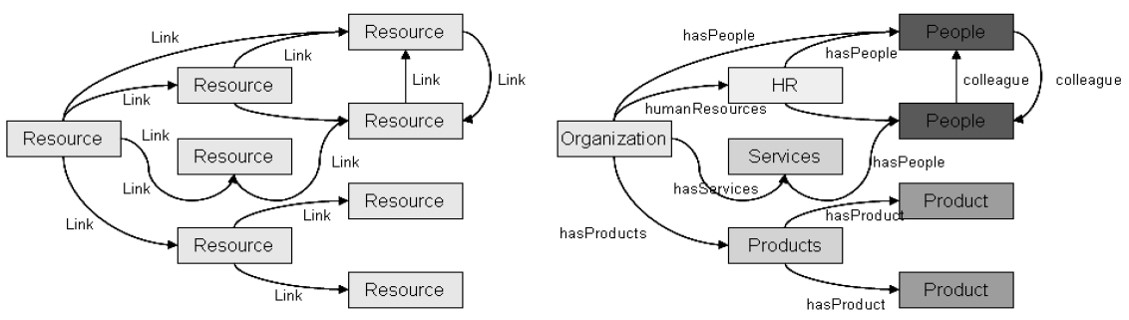
\includegraphics[scale=0.4]{SemanticWeb.jpg}%
%%\caption{Rysunek z \cite{Cardoso2007}}
%\end{figure}
%%

\subsection{Założenia konstrukcyjne logik opisowych}
%
\begin{itemize}
\item Logika opisowa konstruuje pojęcia (\emph{concepts}) i za pomocą tych pojęć opisuje przedmioty indywidualne.
%
\item Pojęcia są budowane z:
\begin{enumerate}
\item pojęć atomicznych (predykatów jednoargumentowych)
\item ról (predykatów binarnych)
\end{enumerate}
%
\item Typ logiki opisowej zależy od zbioru dostępnych sposobów konstrukcji pojęć złożonych z pojęć atomicznych i ról.
%
\item Wiedza dotycząca pojęć i indywiduów może być wyprowadzona automatycznie. W szczególności, możemy ``dowiadywać się'' o relacji subsumpcji pomiędzy pojęciami.
\end{itemize}
%

\subsection{Pudełka semantyczne}
%
\begin{enumerate}
\item TBox - opis terminologii
\begin{itemize}
\item Każdy człowiek jest zwierzęciem.
\item Każde zwierzę ma duszę.
\item Dusza każdego człowieka jest niematerialna.
\end{itemize}
%
\item ABox - opis świata
\begin{itemize}
\item Jan jest człowiekiem.
\item Burek jest zwierzęciem, ale nie jest człowiekiem.
\item Warszawa nie jest zwierzęciem.
\end{itemize}
\end{enumerate}
%

\subsection{Logika opisowa $\mathcal{ALC}$}

\subsection{Logika opisowa $\mathcal{ALC}$}
%
\begin{itemize}
\item język
\item model
\item tablice semantyczne
\end{itemize}
%


\subsection{Alfabet $\mathcal{ALC}$}
%
\begin{definicja}
\label{alfabet (ALC)}
Alfabet $\mathcal{ALC}$ zawiera:%
\begin{enumerate}
\item zbiór stałych indywidualnych $\mathbb{CONST} := \{a_{1}, a_{2}, \dots\},$
%
\item zbiór predykatów %
\begin{itemize}
\item jednoargumentowych (\emph{pojęć atomicznych}):
$$\mathbb{CONCEPT} := \{\top, A_{1}, A_{2}, \dots\}$$%
\item dwuargumentowych (\emph{ról}):
$$\mathbb{ROLE} := \{R_{1}, R_{2}, \dots\}$$
\end{itemize}
%
\item funktory (nazwotwórcze od argumentów nazwowych): $-$, $\sqcap$;
%
\item ``kwantyfikatory'': $\exists .$, $\forall .$;
%
\item funktory (zdaniotwórcze od argumentów nazwowych): $\sqsubseteq$, $=$;
%
\item nawiasy: (, ).
\end{enumerate}
\end{definicja}
%

\subsection{``Kwantyfikatory'' w logikach opisowych}
%
\begin{itemize}
\item $\exists R . C$ - (predykat reprezentujący) zbiór takich przedmiotów, które są powiązane relacją $R$ z \emph{przynajmniej jednym} przedmiotem ze zbioru $C$
$$\exists R . C(x) \equiv \exists y [R(x, y) \land C(y)]$$
%
\item $\forall R . C$ - (predykat reprezentujący) zbiór takich przedmiotów, które są powiązane relacją $R$ \emph{tylko} z przedmiotami ze zbioru $C$
$$\forall R . C(x) \equiv \forall y [R(x, y) \to C(y)]$$
%
\item przykłady:
\begin{itemize}
\item $R$ - jest potomkiem, $C$ - jest Polakiem
\begin{itemize}
\item $\exists R . C$ - potomkowie (jakichś) Polaków
\item  $\forall R . C$ - prawdziwi Polacy (potomkowie tylko Polaków)
\end{itemize}
%
\item $R$ - zna, $C$ - jest celebrytą
\begin{itemize}
\item $\exists R . C$ - ci, którzy znają jakiegoś celebrytę
\item $\forall R . C$ - ci, którzy znają tylko celebrytów
\end{itemize}
\end{itemize}
\end{itemize}
%

\subsection{Zbiór pojęć logiki $\mathcal{ALC}$}
%
Dowolny ciąg elementów alfabetu $\mathcal{ALC}$ jest \emph{napisem} logiki $\mathcal{ALC}$.
%
\begin{definicja}
\label{CONCEPTAL}
Zbiór pojęć logiki $\mathcal{ALC}$ jest najmniejszym zbiorem napisów $\mathcal{ALC}$ spełniającym poniższe warunki:
%
\begin{enumerate}
\item Każde pojęcie atomiczne jest pojęciem $\mathcal{ALC}$.
%
\item Jeżeli $\delta$ jest pojęciem, to $- \delta$ jest pojęciem.
%
\item Jeżeli $\delta_{1}, \delta_{2}$ są pojęciami, to $\delta_{1} \sqcap \delta_{2}$ jest pojęciem.
%
\item Jeżeli $\rho$ jest rolą i $\delta$ jest pojęciem, to $\exists \rho. \delta$ oraz $\forall \rho . \delta$ są pojęciami.
\end{enumerate}
\end{definicja}
%

\subsection{Zbiór pojęć logiki $\mathcal{ALC}$ - przykłady}
%
$HumanBeing$, $Female$, $Polish$, $\top$\\
%
$$Female \sqcap Polish$$
%
$$- HumanBeing$$
%
$$Female \sqcap HumanBeing$$
%
$$- \top$$
%
$$-(Female \sqcap Polish)$$
%

\subsection{Zbiór pojęć logiki $\mathcal{ALC}$ - przykłady (2)}
%
$$\exists hasChild . \top$$
%
$$\forall hasHair . - \top$$
%
$$Female \sqcap (\exists hasChild . \top)$$
%
$$(- Female) \sqcap HumanBeing \sqcap (\exists hasChild . \top) \sqcap \forall hasHair . - \top$$
%

\subsection{Język logiki $\mathcal{ALC}$}
%
\begin{definicja}
\label{PZWAL}
Zbiór poprawnie zbudowanych wyrażeń logiki $\mathcal{ALC}$ jest najmniejszym zbiorem napisów $\mathcal{ALC}$ spełniającym warunek:
%
\begin{enumerate}
%\item Jeżeli $\rho^{(s_{n})} \in \mathbb{PRED}$, a $\delta_{1}, \delta_{2}, \dots, \delta_{s_{n}} \in \mathbb{VAR} \cup \mathbb{CONST}$, to $\rho^{(s_{n})}(\delta_{1}, \delta_{2}, \dots, \delta_{s_{n}}) \in \PZWWRP$.
%%
\item Jeśli $\delta_{1}, \delta_{2}$ są pojęciami logiki $\mathcal{ALC}$, to $\delta_{1} \sqsubseteq \delta_{2}$ oraz $\delta_{1} = \delta_{2}$ są poprawnie zbudowanymi wyrażeniami $\mathcal{ALC}$.%
\item Jeśli $\rho_{1}, \rho_{2}$ są rolami logiki $\mathcal{ALC}$, to $\rho_{1} \sqsubseteq \rho_{2}$ oraz $\rho_{1} = \rho_{2}$ są poprawnie zbudowanymi wyrażeniami $\mathcal{ALC}$.%
\item Jeśli $\delta$ jest pojęciem a $\alpha$ stałą, logiki $\mathcal{ALC}$, to $\delta(\alpha)$ jest poprawnie zbudowanym wyrażeniem $\mathcal{ALC}$.%
\item Jeśli $\rho$ rolą, a $\alpha_{1}$ i $\alpha_{2}$, stałymi logiki $\mathcal{ALC}$,to $\rho(\alpha_{1}, \alpha_{2})$ jest poprawnie zbudowanym wyrażeniem $\mathcal{ALC}$.%
\end{enumerate}
Zbiór wyrażeń spełniających warunki 1 lub 2 jest nazywany pudełkiem terminologicznym.\\ %
Zbiór wyrażeń spełniających warunki 3 lub 4 jest nazywany pudełkiem asercji.
\end{definicja}
%

\subsection{Język logiki $\mathcal{ALC}$ - przykłady (2)}
%
$$Male \sqsubseteq Animal$$
%
$$Female \sqsubseteq - Animal$$
%
$$Man = HumanBeing \sqcap - Female$$ 
%
$$Father = Man \sqcap \exists hasChild . \top$$
%
$$Bachelor = Man \sqcap \forall hasSpouse . - \top$$
%
$$\exists hasChild . \top \sqsubseteq \exists hasSpouse . \top$$
%
$$GenuineMan = Man \sqcap (\exists build . House) \sqcap (\exists hasChild . Male) \sqcap (\exists plant .Tree)$$
%


\subsection{Język logiki $\mathcal{ALC}$ - przykłady (2)}
%
\begin{quote}
\dots\\
Podobno każdy ma swój kawałek cienia - \\
brak cienia jest dowodem nieistnienia - \\
lecz bez kawałka światła \\
nie jest łatwo \dots (G. Turnau, \emph{Kawałek cienia})
\end{quote}
%
$$\top \sqsubseteq \exists hasShadow . \top$$
(zainspirowany przez J. Pogonowskiego) \\
%

\subsection{Język logiki $\mathcal{ALC}$ - przykłady (3)}
%
$$hasChild \sqsubseteq hasDescendant$$
%
$$hasWife = hasHusband$$
%

\subsection{Język logiki $\mathcal{ALC}$ - przykłady (4)}
%
$HumanBeing(Jan)$\\
%
$\top(Jan)$\\
%
$$(Female \sqcap Polish)(Jan)$$
%
$$(- HumanBeing)(Burek)$$
%
$$(\exists hasChild . \top)(Jan)$$
%
$$(\forall hasHair . - \top)(Jan)$$
%
$$(Female \sqcap (\exists hasChild . \top))(Anna)$$
%
$$((- Female) \sqcap HumanBeing \sqcap (\exists hasChild . \top) \sqcap \forall hasHair . - \top)(Jan)$$
%

\subsection{Czego nie można powiedzieć w $\mathcal{ALC}$?}
%
\begin{itemize}
	\item Nie istnieje największa liczba pierwsza.
	\item Każdy kij ma dwa końce.
	\item Przyjaciele moich przyjaciół są moimi przyjaciółmi.
\end{itemize}
%

\subsection{Modele $\mathcal{ALC}$}
%
\begin{definicja}
Parę $\mathfrak{M} = <\mathbb{D}, \mathbb{I}>$ nazywamy modelem dla języka $\mathcal{ALC}$ jeżeli:
%
\begin{enumerate}
\item $\mathbb{D} \neq \emptyset$,
%
\item $\mathbb{I}$ jest taką funkcją, która:
%
\begin{enumerate}
\item odwzorowuje zbiór $\mathbb{CONST}$ w zbiór $\mathbb{D}$,
%
\item odwzorowuje zbiór pojęć w $\wp(\mathbb{D})$, przy czym spełnione są następujące warunki:
$$\mathbb{I}(\top) = \mathbb{D}$$
%$$\mathbb{I}(\bot) = \emptyset$$
$$\mathbb{I}(- \delta) = \mathbb{D}\setminus \mathbb{I}(\delta)$$
$$\mathbb{I}(\delta_{1} \sqcap \delta_{2}) = \mathbb{I}(\delta_{1}) \cap \mathbb{I}(\delta_{2})$$
$$\mathbb{I}(\exists \rho . \delta) = \{x \in \mathbb{D} : \exists y <x, y> \in \mathbb{I}(\rho) \land y \in \mathbb{I}(\delta)]\}$$
 %(=zbiór wszystkich podzbiorów $\mathbb{D}$),\}$$
$$\mathbb{I}(\forall \rho . \delta) = \{x \in \mathbb{D} : \forall y [<x, y> \in \mathbb{I}(\rho) \to y \in \mathbb{I}(\delta)]\}$$
 %(=zbiór wszystkich podzbiorów $\mathbb{D}$),
%
\item odwzorowuje zbiór ról  w $\wp(\mathbb{D} \times \mathbb{D})$. %(=zbiór wszystkich podzbiorów iloczynu kartezjańskiego $\mathbb{D}$ ``razy'' $\mathbb{D}$)
\end{enumerate}
\end{enumerate}
\end{definicja}
%


\subsection{Spełnianie w $\mathcal{ALC}$}
%
\begin{eqnarray}
\label{sat-AL}
& \mathfrak{M} \vDash \delta(\alpha) \equiv \mathbb{I}(\alpha) \in \mathbb{I}(\delta) \\
%
& \mathfrak{M} \vDash \rho(\alpha_1, \alpha_2) \equiv <\mathbb{I}(\alpha_1), \mathbb{I}(\alpha_2)> \in \mathbb{I}(\rho) \\
%
& \mathfrak{M} \vDash \epsilon_{1} \sqsubseteq \epsilon_{2} \equiv \mathbb{I}(\epsilon_{1}) \subseteq \mathbb{I}(\epsilon_{2}) \\
%
& \mathfrak{M} \vDash \epsilon_{1} \equiv \epsilon_{2} \equiv \mathbb{I}(\epsilon_{1}) = \mathbb{I}(\epsilon_{2})
\end{eqnarray}
%
gdzie: $\epsilon_{1}, \epsilon_{2}$ reprezentują nazwy pojęć \emph{lub} ról.
%

\subsection{Spełnianie w $\mathcal{ALC}$~(2)}
%
\begin{equation}
\vDash \phi \equiv \forall \mathfrak{M}~ \mathfrak{M}\vDash \phi.
\end{equation}
%

\subsection{Spełnianie w $\mathcal{ALC}$~(3)}
%
\begin{equation}
\mathfrak{M} \vDash \Delta \equiv \forall \phi \in \Delta ~\mathfrak{M} \vDash \phi.
\end{equation}
%

\subsection{Spełnianie w $\mathcal{ALC}$~(4)}
%
\begin{eqnarray}
\delta \text{ jest spełnialne ze względu na pudełko terminologiczne } \Delta \equiv \nonumber \\ 
\text{ istnieje taki model } \mathfrak{M}=<\mathbb{D}, \mathbb{I}> \text{ że, } \mathfrak{M}\vDash \Delta \text{ oraz } \mathbb{I}(\delta) \neq \emptyset.
\end{eqnarray}
%

\subsection{Spełnianie w $\mathcal{ALC}$~(5)}
%
\begin{fakt}
$\vDash \delta_{1} \sqsubseteq \delta_{2}$ wtedy i tylko wtedy, gdy dla dowolnego pudełka terminologicznego $\Delta$, $\delta_1 \sqcap - \delta_1$ nie jest spełnialne ze względu na $\Delta$.
\end{fakt}
%

\subsection{Metoda tablic analitycznych w $\mathcal{ALC}$ -- krok po kroku}
Czy $\delta_{1} \sqsubseteq \delta_{2}$ jest prawem logiki?
%
\begin{enumerate}
\item Utwórz pojęcie  $\delta_1 \sqcap - \delta_2$
%
%\item Przekształcić $\delta_1 \sqcap - \delta_2$ do negacyjnej postaci normalnej $\delta^{\#}$.
%%
\item Wstaw $(\delta_1 \sqcap - \delta_2)(\alpha)$ jako korzeń tablicy analitycznej $T$ (dla dowolnej stałej $\alpha$)!
%
\item Korzystając z atomowych tablic analitycznych zredukuj $T$!
%
\item Czy $T$ jest zamknięta?
%
\begin{itemize}
\item \textcolor[rgb]{0.00,1.00,0.00}{TAK}, $\delta_{1} \sqsubseteq \delta_{2}$ \textcolor[rgb]{0.00,1.00,0.00}{jest} prawem logiki.
%
\item \textcolor[rgb]{1.00,0.00,0.00}{NIE}, $\delta_{1} \sqsubseteq \delta_{2}$ \textcolor[rgb]{0.98,0.00,0.00}{nie jest} prawem logiki.
\end{itemize}
\end{enumerate}
%

\subsection{Zamknięte i otwarte tablice analityczne w logikach opisowych}
%
\begin{definicja}
Tablice analityczna jest \emph{zamknięta}, jeżeli każda jej gałąź:
\begin{enumerate}
\item zawiera dwa wyrażenia sprzeczne: $\delta(\alpha)$, $(- \delta)(\alpha)$;
\item lub zawiera wyrażenie $(- \top)(\alpha)$.
\end{enumerate}
Tablice analityczna jest \emph{otwarta}, jeżeli nie jest zamknięta.
\end{definicja}
%

%\subsection{Negacyjna postać normalna}
%\begin{definicja}
%Wyrażenie $\phi$ ma \emph{negacyjną postać normalną}, gdy funktor negacji łączy tylko pojęcia atomiczne lub pojęcia zbudowane za pomocą pojęć atomicznych oraz funktorów: $-$ lub $\sqcap$.
%\end{definicja}	
%%

%\subsection{Reguły transformacji do negacyjnej postaci normalnej}
%\begin{table}[p]
%\begin{center}
%\begin{tabular}{|c|c|}
%\hline
%\bf{Przed} & \bf{Po}\\
%\hline
%$- \forall R . \delta$ & $\exists R . - \delta$ \\
%\hline
%$- \exists R . \delta$ & $\forall R . - \delta$ \\
%\hline
%\end{tabular}
%\caption{Redukcja nawiasów w wyrażeniach \KRZ}
%\label{RedukcjaPZWKRZ}
%\end{center}
%\end{table}
%%

\subsection{Tablice analityczne w $\mathcal{ALC}$}
%
\begin{itemize}
\item $\mathbb{TON}$: \Tree [.{$\boldsymbol{- - \delta(\alpha)}$} {$\delta(\alpha)$} ]
\end{itemize}
%

\subsection{Tablice analityczne w $\mathcal{ALC}~(2)$}
%%
%\begin{itemize}
%\item $\mathbb{TOK}$: \Tree [.{$\boldsymbol{(\delta_1  \sqcap \delta_2)(\alpha)}$} [.{$\delta_{1} (\alpha)$} [.{$\delta_{2} (\alpha)$} ] ] ]
%%
%\item $\mathbb{TONK}$: \Tree [.{$\boldsymbol{-(\delta_1  \sqcap \delta_2)(\alpha)}$} {$(- \delta_{1}) (\alpha)$} {$(- \delta_{2}) (\alpha)$} ]
%\end{itemize}
%%

\subsection{Tablice analityczne w $\mathcal{ALC}$~(3)}
%
\begin{itemize}
\item $\mathbb{TO}\exists$: \Tree [.{$\boldsymbol{(\exists R . \delta)(\alpha)}$} [.{$R (\alpha, \beta)$} [.{$\delta (\beta)$} ] ] ]\\
gdzie: $\beta$ jest nową stałą.\\
%
\item $\mathbb{TO}\forall$: \Tree [.{$\boldsymbol{(\forall R . \delta)(\alpha)}$} [.{\boldsymbol{$R (\alpha, \beta)}$} [.{$\delta (\beta)$} ] ] ]\\
gdzie: $\beta$ jest dowolną stałą.
\end{itemize}
%

\subsection{Tablice analityczne w $\mathcal{ALC}$~(4)}
%
\begin{itemize}
\item $\mathbb{TON}\exists$: \Tree [.{$\boldsymbol{(- \exists R . \delta)(\alpha)}$} [.{$(\forall R . - \delta)(\alpha)$} ] ] ]\\
%gdzie: $\alpha$ jest dowolną stałą.\\
%
\item $\mathbb{TON}\forall$: \Tree [.{$\boldsymbol{(- \forall R . \delta)(\alpha)}$} [.{$(\exists R . - \delta)(\alpha)$} ] ] ]\\
%gdzie: $\alpha$ jest dowolną stałą.
\end{itemize}
%

\subsection{Metoda tablic analitycznych w $\mathcal{ALC}$ -- krok po kroku (2)}
Czy $\delta_{1} = \delta_{2}$ jest prawem logiki?
%
\begin{enumerate}
\item Utwórz pojęcia:  $\delta_1 \sqcap - \delta_2$ oraz $\delta_2 \sqcap - \delta_1$
%
%\item Przekształcić $\delta_1 \sqcap - \delta_2$ do negacyjnej postaci normalnej $\delta^{\#}$.
%%
\item Wstaw $(\delta_1 \sqcap - \delta_2)(\alpha)$ i $(\delta_2 \sqcap - \delta_1)(\alpha)$ jako korzenie dwóch tablic analitycznych $T_1$ i $T_2$ (dla dowolnej stałej $\alpha$)!
%
\item Korzystając z atomowych tablic analitycznych zredukuj obie tablice!
%
\item Czy $T_1$ i $T_2$ są (zarazem) zamknięte?
%
\begin{itemize}
\item \textcolor[rgb]{0.00,1.00,0.00}{TAK}, $\delta_{1} = \delta_{2}$ \textcolor[rgb]{0.00,1.00,0.00}{jest} prawem logiki.
%
\item \textcolor[rgb]{1.00,0.00,0.00}{NIE}, $\delta_{1} = \delta_{2}$ \textcolor[rgb]{0.98,0.00,0.00}{nie jest} prawem logiki.
\end{itemize}
\end{enumerate}
%

\subsection{Metoda tablic analitycznych w $\mathcal{ALC}$ -- krok po kroku (3)}
Czy $\delta(\alpha)$ jest prawem logiki?
%
\begin{enumerate}
\item Wstaw $(- \delta)(\alpha)$ jako korzeń tablicy analitycznej $T$!
%
\item Korzystając z atomowych tablic analitycznych zredukuj $T$!
%
\item Czy $T$ jest zamknięta?
%
\begin{itemize}
\item \textcolor[rgb]{0.00,1.00,0.00}{TAK}, $\delta(\alpha)$ \textcolor[rgb]{0.00,1.00,0.00}{jest} prawem logiki.
%
\item \textcolor[rgb]{1.00,0.00,0.00}{NIE}, $\delta(\alpha)$ \textcolor[rgb]{0.98,0.00,0.00}{nie jest} prawem logiki.
\end{itemize}
\end{enumerate}
%

\subsection{Metoda tablic analitycznych w $\mathcal{ALC}$ -- krok po kroku (4)}
%
Czy $\rho_{1} \sqsubseteq \rho_{2}$ i $\rho_{1} \equiv \rho_{2}$ są prawami logiki?\\
%
Czy $\rho(\alpha_{1},\alpha_{2})$ jest prawem logiki?
%

\subsection{Reprezentacja relacji w logice}

\subsection{Relacje w życiu i w logice}
%
\begin{center}
\begin{table}
{\scriptsize
\begin{tabular}{|c|c|c|}
\hline
miłość & $x$ kocha $y$ & Jan kocha Annę.\\
\cline{3-3}
& & Tomasz kocha Ewę.\\
\cline{3-3}
& & Tomasz kocha Annę.\\
\cline{3-3}
& & Tomasz kocha Jana. \\
\cline{3-3}
& & \dots \\
\hline
ojcostwo & $x$ spłodził $y$ & Jan spłodził Zofię.\\
\cline{3-3}
& & \dots \\
\hline
bycie większym & $x$ jest większe niż $y$ & \dots \\
\hline
bycie dłużnikem & $x$ jest dłużnikiem $y$ & \dots \\
\hline
pożyczanie pieniędzy & $x$ pożyczył od $y$ $z$ zł & Jan pożyczył od Tomasza 100 zł. \\
\hline
\end{tabular}
}
\end{table}
\end{center}
%

\subsection{Reprezentacja relacji w \WRP}
%
\begin{itemize}
\item $P(x, y)$:
\begin{enumerate}
\item $x$ kocha $y$
\item $x$ spłodził $y$
\item $x$ jest większe niż $y$
\item $x$ jest dłużnikiem $y$
\item \dots
\end{enumerate}
%
\item $R(x, y, z)$:
\begin{enumerate}
\item  $x$ pożyczył od $y$ sumę $z$ zł
\item \dots
\end{enumerate}
\end{itemize}
%

\subsection{Reprezentacja relacji w modelach \WRP}
%
\begin{itemize}
\item relacje dwuargumentowe są zbiorami par (uporządkowanych)
%
\item relacje trzyargumentowe są zbiorami trójek (uporządkowanych)
%
\item \dots
\item relacje $n$-argumentowe są zbiorami $n$-tek (uporządkowanych)
\end{itemize}
%

\subsection{Obrazkowa teoria relacji}
\begin{center}
<1>{
\begin{figure}
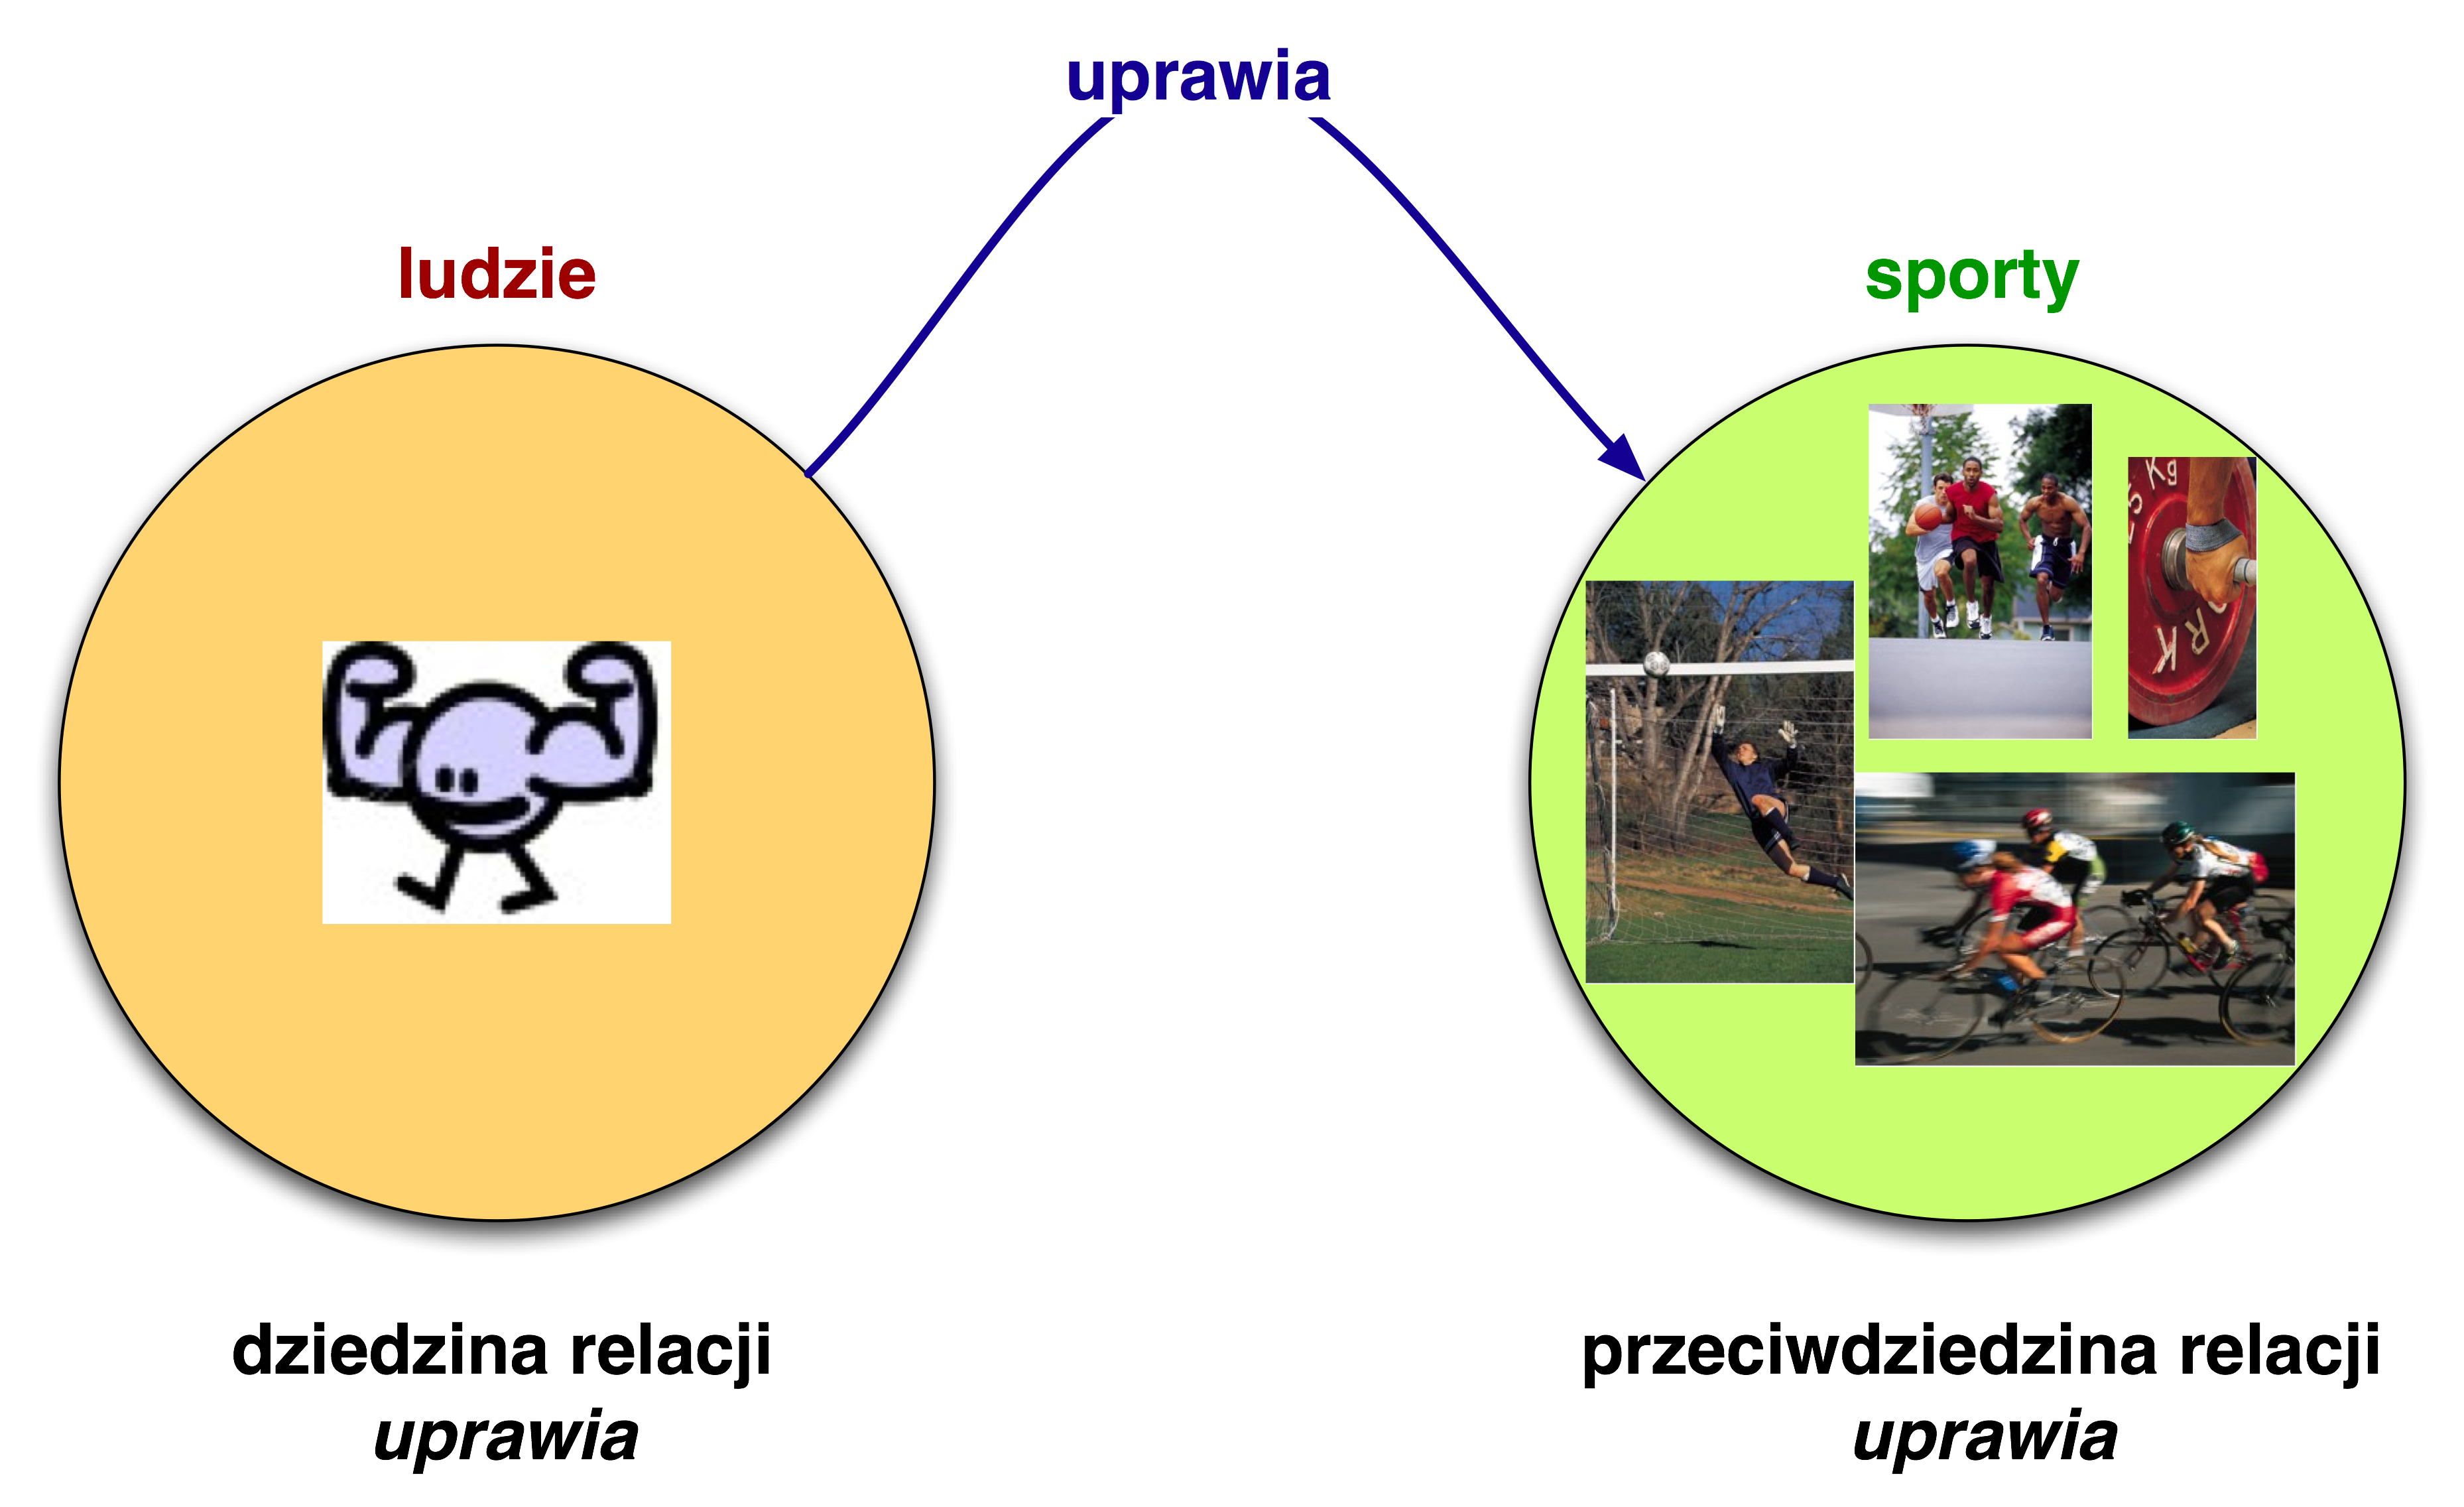
\includegraphics[scale=0.35]{../pliki_wlasne/domainrange.jpg}
\caption{Dziedzina i przeciwdziedzina relacji}
\end{figure}
}
<2>{
\begin{figure}
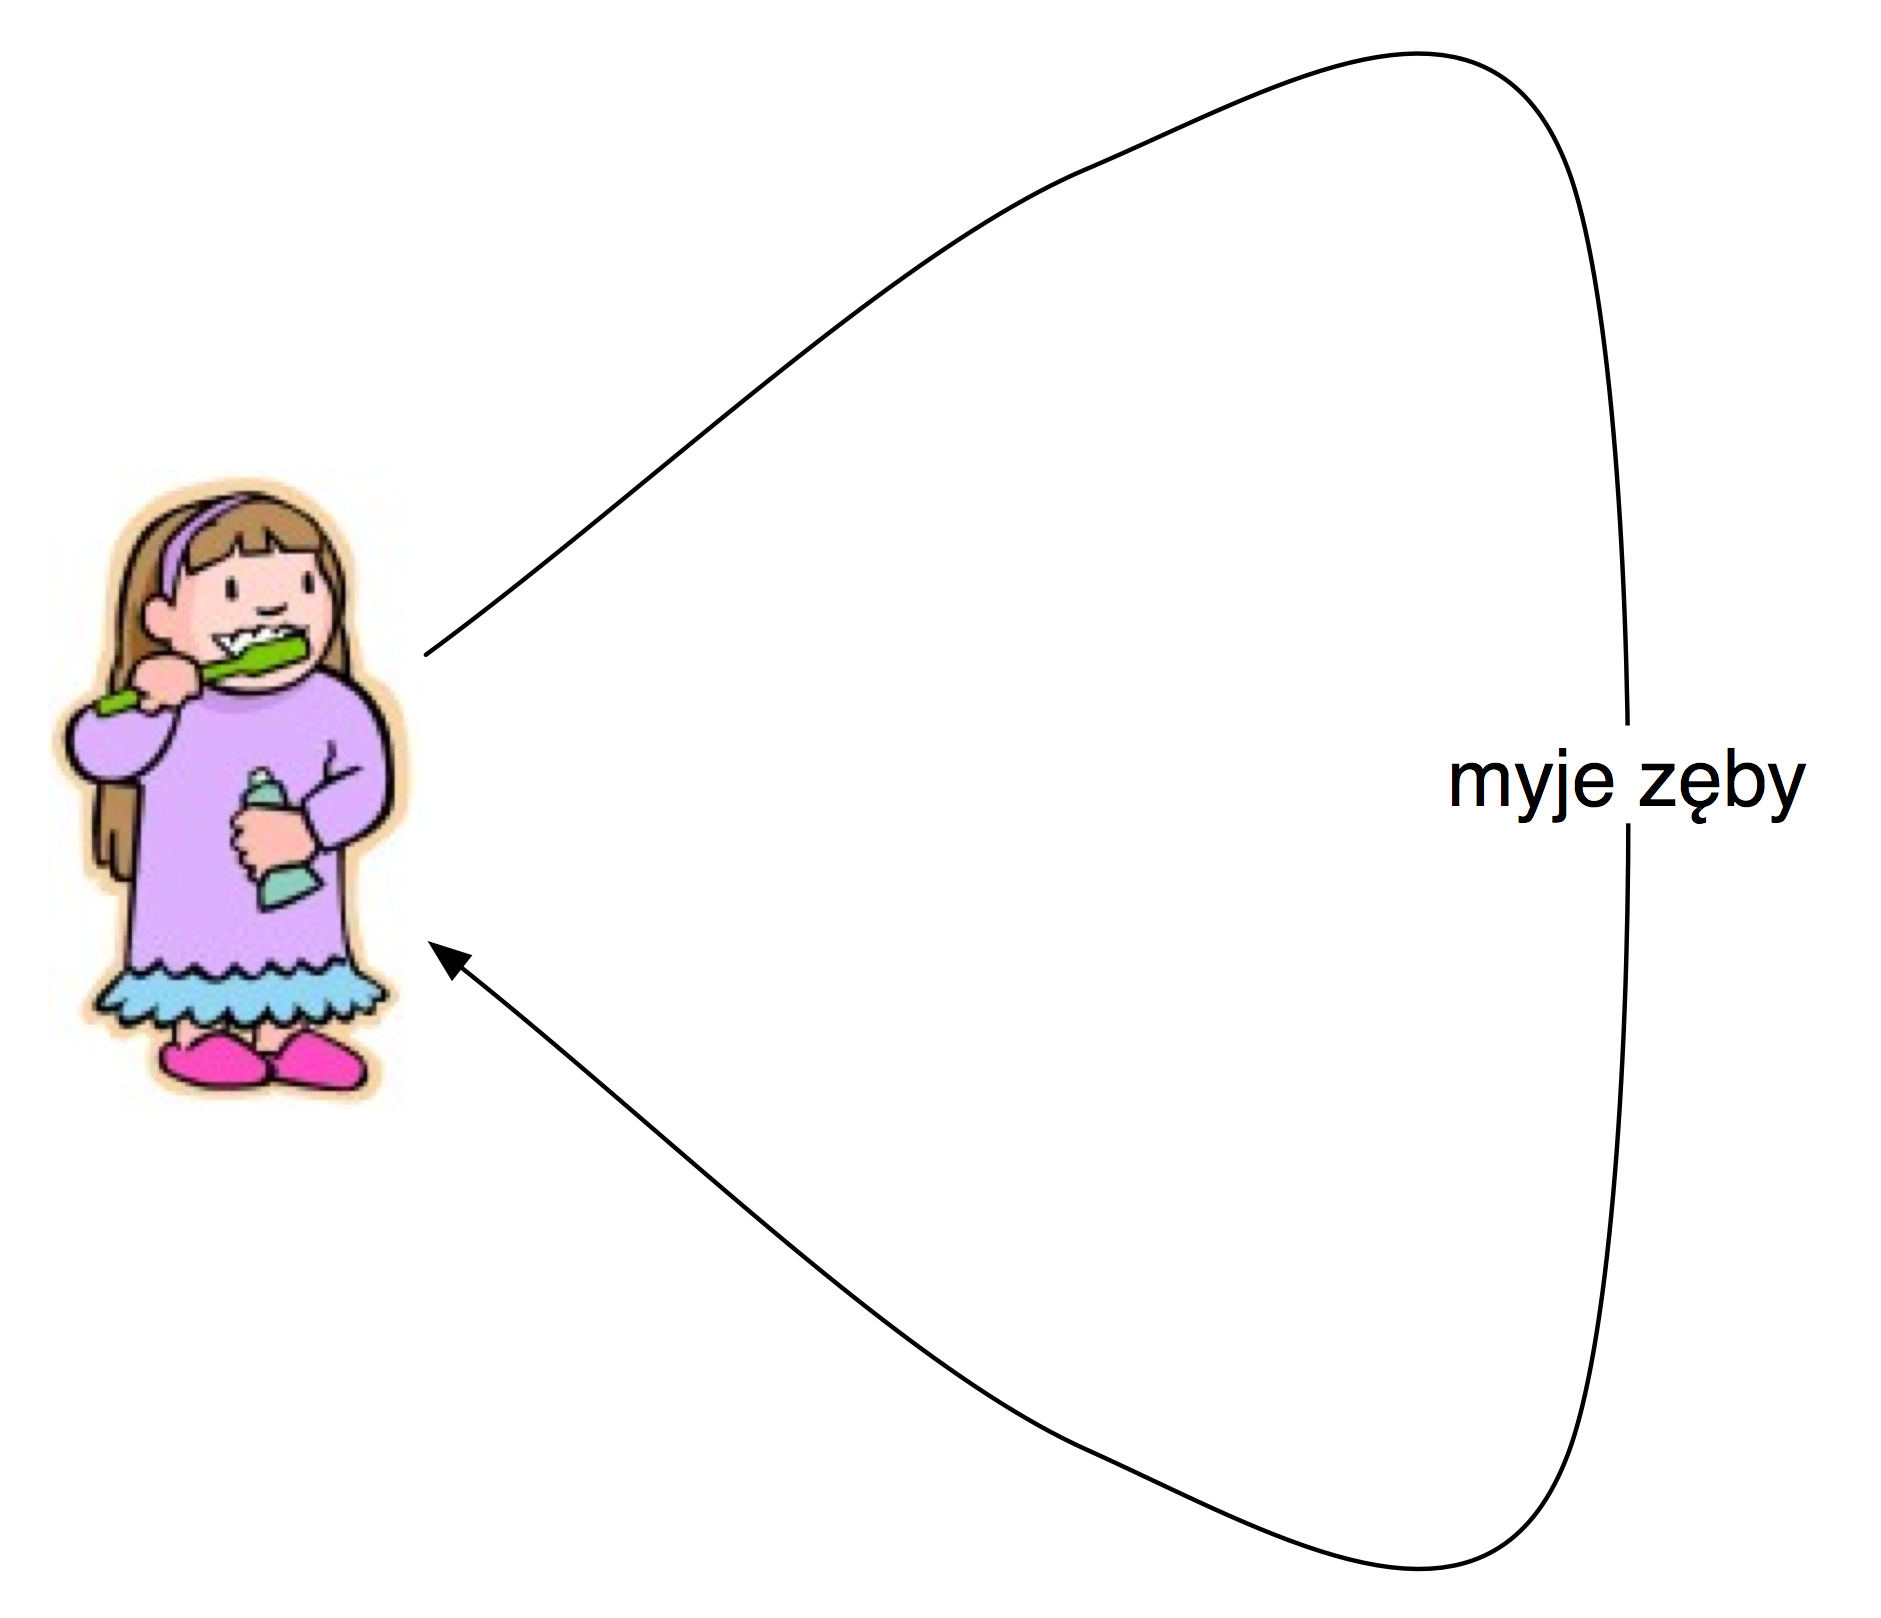
\includegraphics[scale=0.45]{../pliki_wlasne/zwrotna.jpg}
\caption{Zwrotność}
\end{figure}
}
<3>{
\begin{figure}
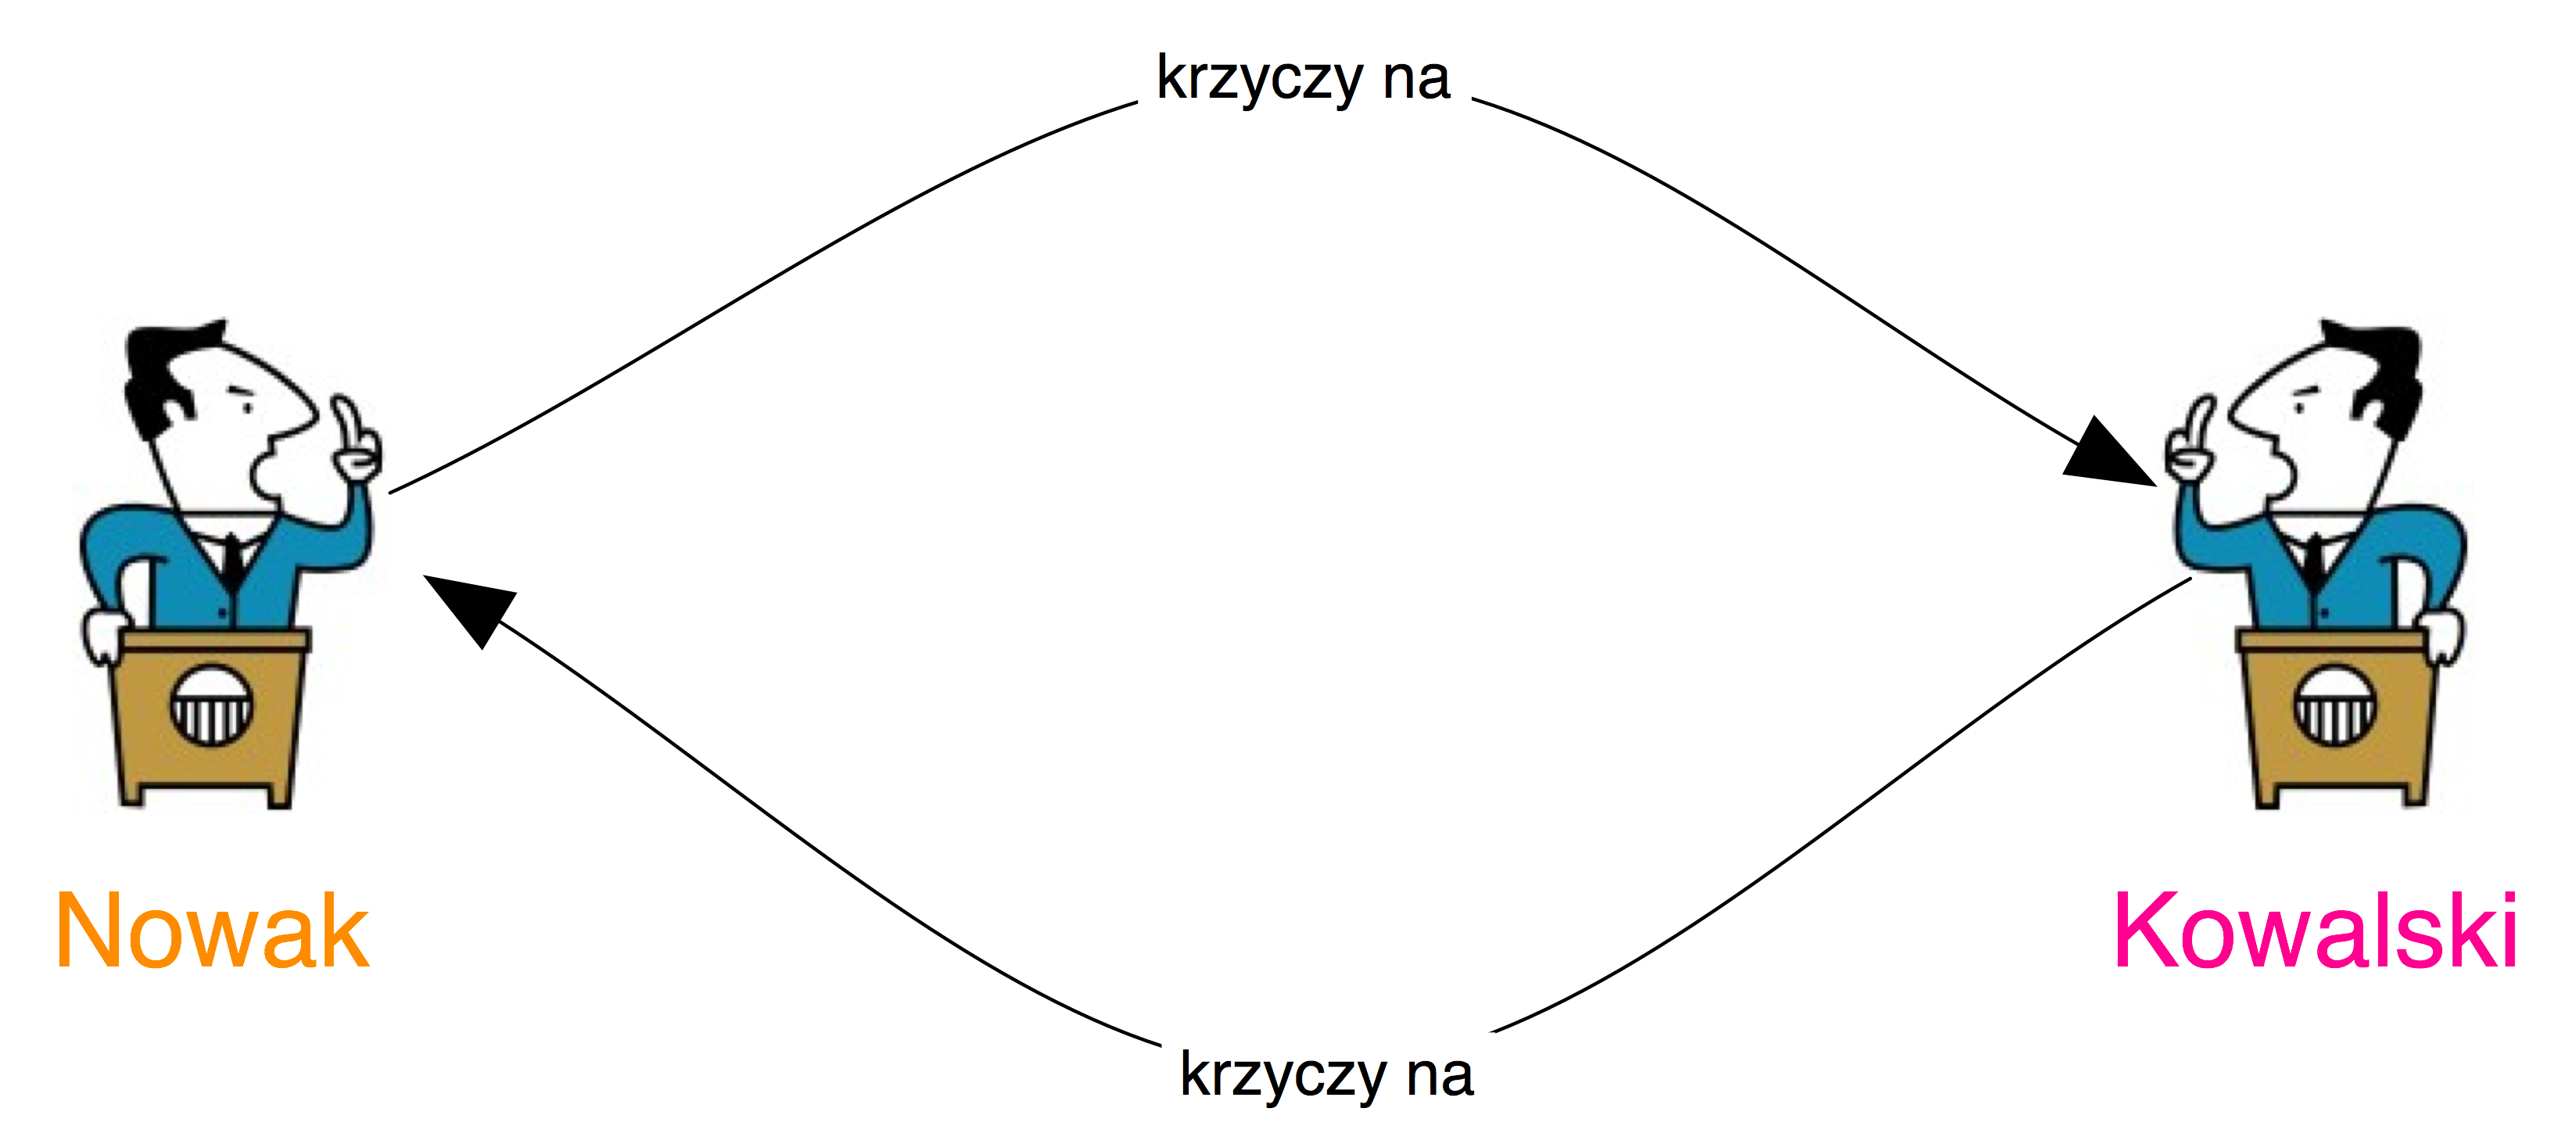
\includegraphics[scale=0.45]{../pliki_wlasne/symetryczna.jpg}
\caption{Symetryczność}
\end{figure}
}
<4>{
\begin{figure}
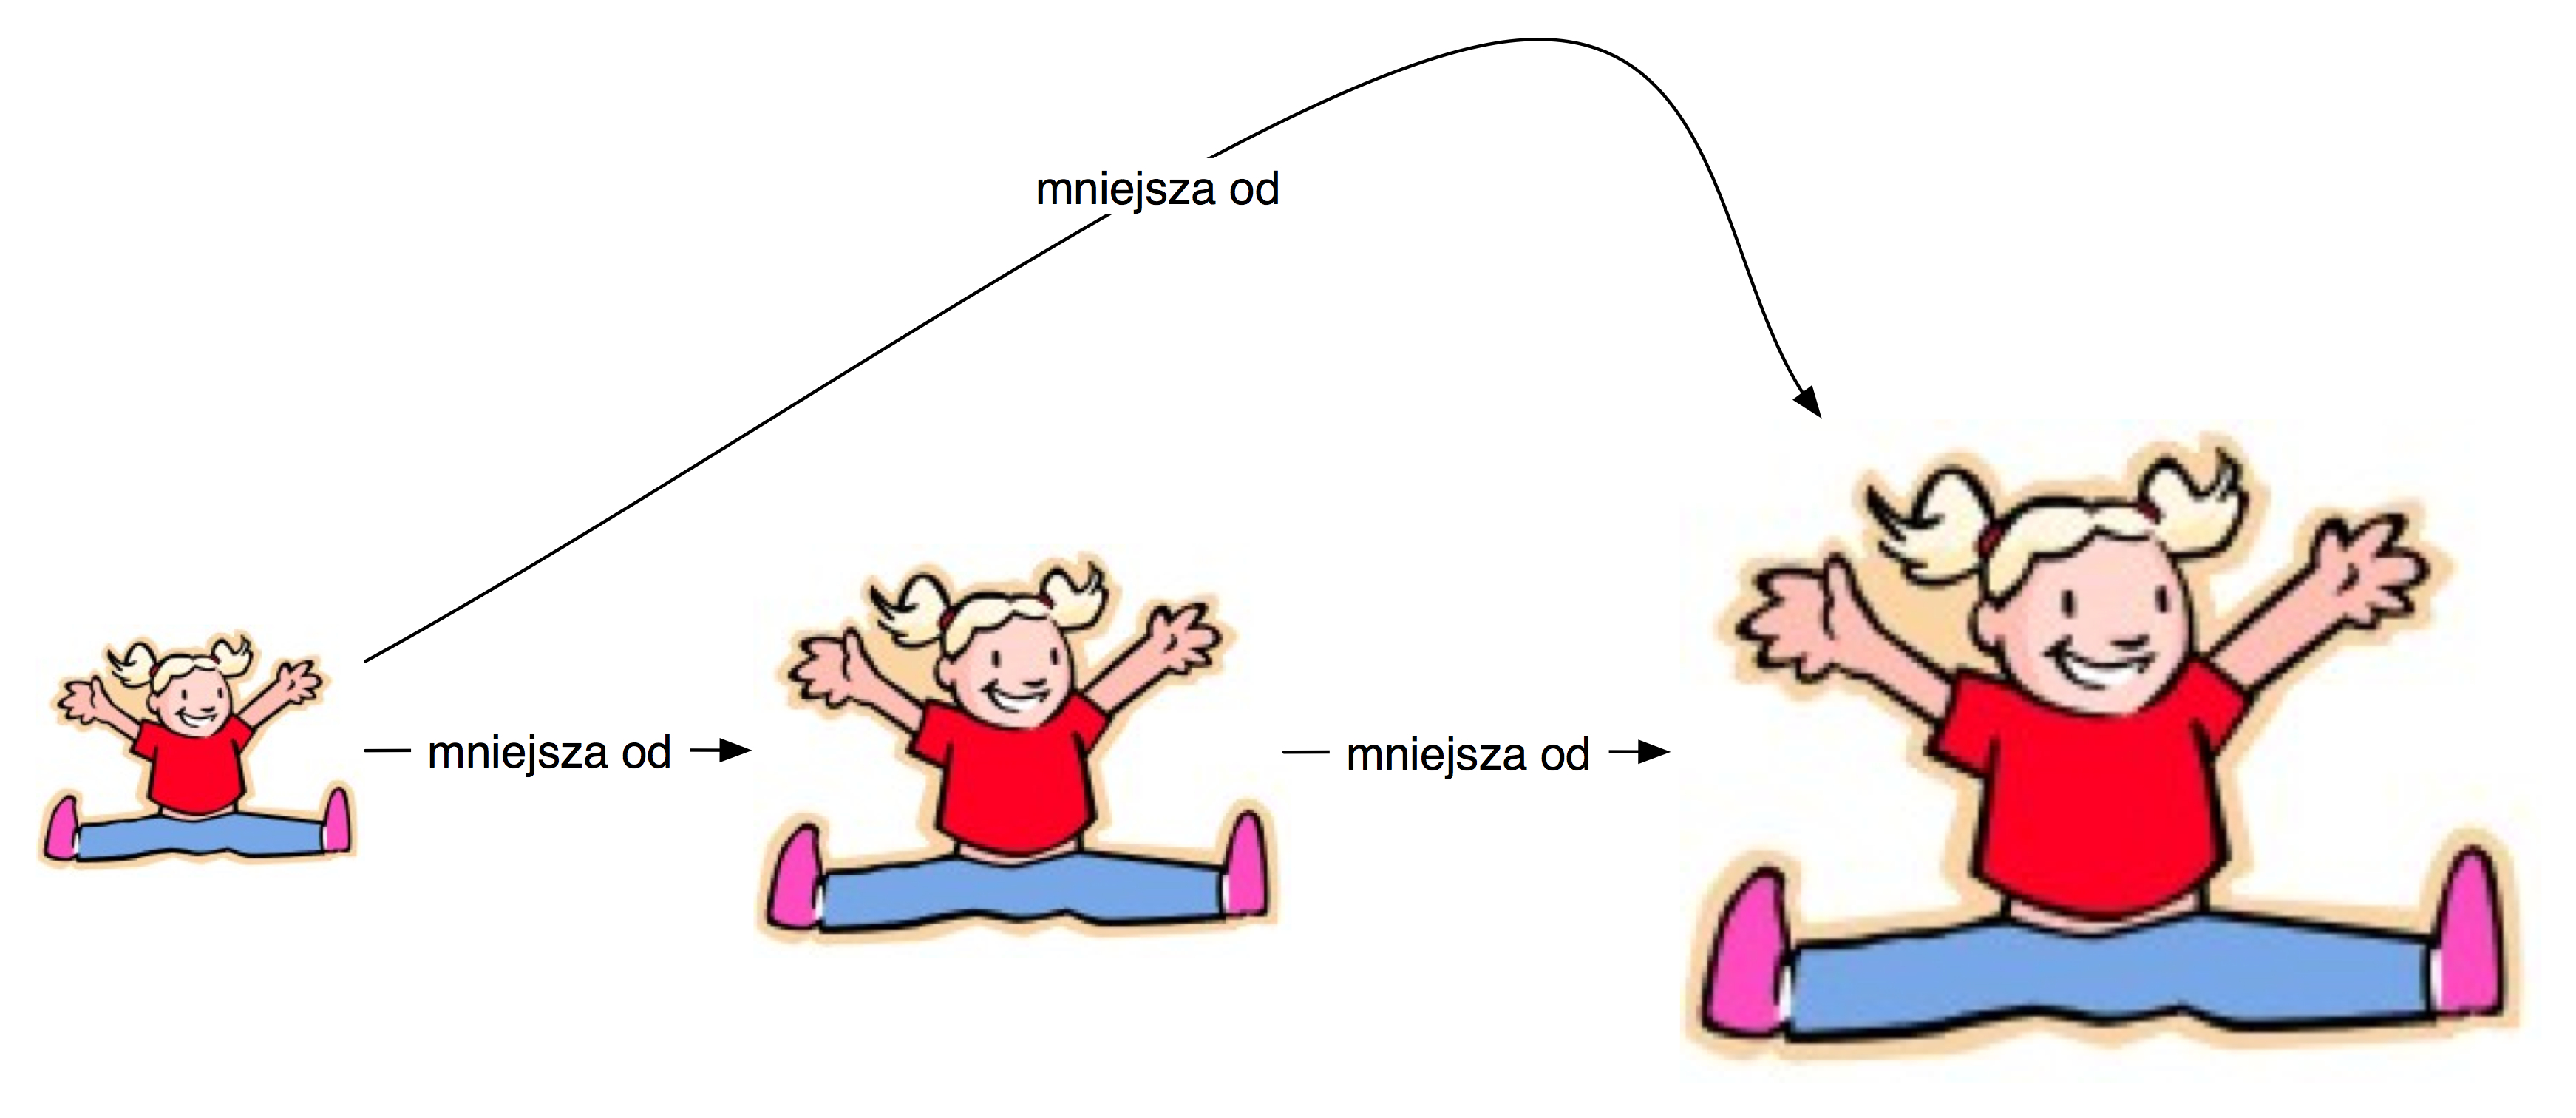
\includegraphics[scale=0.45]{../pliki_wlasne/przechodnia.jpg}
\caption{Przechodność}
\end{figure}
}
\end{center}
%



\subsection{Dziedzina i przeciwdziedzina relacji}
%
\begin{definicja}
Jeżeli $R$ jest relacją dwuargumentową, to $x$ należy do \emph{dziedziny} relacji $R$ wtedy i tylko wtedy, gdy $$\exists y~ R(x, y).$$
\end{definicja}
%
\begin{definicja}
Jeżeli $R$ jest relacją dwuargumentową, to $x$ należy do \emph{przeciwdziedziny} relacji $R$ wtedy i tylko wtedy, gdy $$\exists y~ R(y, x).$$
\end{definicja}
%

\subsection{Dziedzina i przeciwdziedzina relacji - przykłady}
%
\begin{center}
\begin{table}
{\small
\begin{tabular}{|c|c|c|}
\hline
\textbf{relacja} & \textbf{dziedzina} & \textbf{przeciwdziedzina} \\
\hline
miłość & (ludzie) kochający & (ludzie) kochani\\
\hline
ojcostwo & ojcowie & (prawie wszyscy) ludzie \\
\hline
bycie dłużnikem & dłużnicy & wierzyciele \\
\hline
\end{tabular}
}
\end{table}
\end{center}
%

\subsection{(Najważniejsze) rodzaje relacji dwuargumentowych}
%
\begin{enumerate}
\item zwrotne i przeciwzwrotne
\item symetryczne, asymetryczne, antysymetryczne
\item przechodnie
\item funkcje
\end{enumerate}
%

\subsection{Relacje zwrotne}
%
\begin{definicja}
Relacja dwuargumentowa $R$ jest \emph{zwrotna} wtedy i tylko wtedy, gdy $$\forall x ~R(x,x).$$
\end{definicja}
%
przykłady:
\begin{enumerate}
\item równoległość (prostych)
\item $=$
\item podobieństwo
\end{enumerate}
%
antyprzykłady:
\begin{enumerate}
\item prostopadłość (prostych)
\item $<$
\item bycie dłużnikiem
\item nienawiść
\end{enumerate}
%

\subsection{Relacje przeciwzwrotne}
%
\begin{definicja}
Relacja dwuargumentowa $R$ jest \emph{przeciwzwrotna} wtedy i tylko wtedy, gdy $$\forall x ~\neg R(x,x).$$
\end{definicja}
%
przykłady:
\begin{enumerate}
\item prostopadłość (prostych)
\item $<$
\item bycie dłużnikiem
\end{enumerate}
antyprzykłady:
\begin{enumerate}
\item równoległość (prostych)
\item $=$
\item podobieństwo
\item nienawiść
\end{enumerate}
%


\subsection{Relacje symetryczne}
%
\begin{definicja}
Relacja dwuargumentowa $R$ jest \emph{symetryczna} wtedy i tylko wtedy, gdy $$\forall x,y ~[R(x,y) \to R(y, x)].$$
\end{definicja}
%
przykłady:
\begin{enumerate}
\item równoległość (prostych)
\item $=$
\item podobieństwo
\item prostopadłość (prostych)
\end{enumerate}
%
antyprzykłady:
\begin{enumerate}
\item $<$
\item bycie dłużnikiem
\end{enumerate}
%

\subsection{Relacje asymetryczne}
%
\begin{definicja}
Relacja dwuargumentowa $R$ jest \emph{asymetryczna} wtedy i tylko wtedy, gdy $$\forall x,y ~[R(x,y) \to \neg R(y, x)].$$
\end{definicja}
%
przykłady:
\begin{enumerate}
\item $<$
\item bycie dłużnikiem
\end{enumerate}
%
antyprzykłady:
\begin{enumerate}
\item równoległość (prostych)
\item prostopadłość (prostych)
\item $=$
\item podobieństwo
\end{enumerate}
%

\subsection{Relacje antysymetryczne}
%
\begin{definicja}
Relacja dwuargumentowa $R$ jest \emph{antysymetryczna} wtedy i tylko wtedy, gdy $$\forall x,y ~[R(x,y) \land R(y, x) \to x=y].$$
\end{definicja}
%
przykłady:
\begin{enumerate}
\item $\leq$
\end{enumerate}
%
antyprzykłady:
\begin{enumerate}
\item równoległość (prostych)
\item prostopadłość (prostych)
\item podobieństwo
\item $<$
\item bycie dłużnikiem
\end{enumerate}
%

\subsection{Relacje przechodnie}
%
\begin{definicja}
Relacja dwuargumentowa $R$ jest \emph{przechodnia} wtedy i tylko wtedy, gdy $$\forall x,y,z ~[R(x,y) \land R(y, z) \to R(x,z)].$$
\end{definicja}
%
przykłady:
\begin{enumerate}
\item równoległość (prostych)
\item $<$
\item $=$
\end{enumerate}
%
antyprzykłady:
\begin{enumerate}
\item prostopadłość (prostych)
\item podobieństwo
\end{enumerate}
%

\subsection{Funkcje}
%
\begin{definicja}
Relacja dwuargumentowa $R$ jest \emph{funkcją} wtedy i tylko wtedy, gdy $$\forall x,y_{1},y_{2} ~[R(x,y_{1}) \land R(x, y_{2}) \to y_{1}=y_{2}].$$
\end{definicja}
%
przykłady:
\begin{enumerate}
\item $=$
\item $x$ urodził się w dniu $y$
\item $x$ ma numer PESEL $y$
\end{enumerate}
%
antyprzykłady:
\begin{enumerate}
\item równoległość (prostych)
\item prostopadłość (prostych)
\item podobieństwo
\item $<$
\item bycie dłużnikiem
\end{enumerate}
%

\subsection{Trzyczynnikowa klasyfikacja relacji  - przykłady}
%
\begin{center}
\begin{table}
\begin{tabular}{|c||c|c|c|}
\hline 
\textbf{relacja} & \textbf{zwrotna} & \textbf{symetryczna}  & \textbf{przechodnia} \\
\hline
podobieństwo & tak & tak & nie \\ 
\hline
$<$ & nie & asymetryczna & tak\\
\hline
bycie dłużnikiem & nie & nie & ??? \\
\hline
\end{tabular}
\end{table}
\end{center}
% 

\subsection{Relacje (ściśle) porządkujące}
%
\begin{definicja}
Relacja jest ściśle porządkująca (jest porządkiem) jeżeli jest asymetryczna i przechodnia.
\end{definicja}
%
przykłady:
\begin{enumerate}
\item $<$
\item być głupszym niż
\end{enumerate}
%
antyprzykłady:
\begin{enumerate}
\item równoległość (prostych)
\item $\leq$
\end{enumerate}
%

\subsection{Relacje równoważnościowe}
%
\begin{definicja}
Relacja jest równoważnościowa jeżeli jest zwrotna, symetryczna i przechodnia.
\end{definicja}
%
przykłady
\begin{enumerate}
\item równoległość (prostych)
\item równoważenie się na wadze ($x$ waży tyle samo, co $y$)
\end{enumerate}
%
antyprzykłady:
\begin{enumerate}
\item $\leq$
\item bycie dłużnikiem
\item być niegłupszym niż
\end{enumerate}
%
Dzięki tzw. twierdzeniu o abstrakcji relacje równoważnościowe mogą służyć do definiowania własności, np.
\begin{enumerate}
\item równoległość definiuje kierunek (prostej)
\item równoważenie się na wadze definiuje ciężar
\end{enumerate}
%

\subsection{Operacje na relacjach}
%
\begin{itemize}
	\item ogólne (teoriomnogościowe): suma, iloczyn, różnica, dopełnienie, itd.
	%
	\item lokalne:
	\begin{enumerate}
		\item inwers relacji
		\item iloczyn względny relacji
	\end{enumerate}
\end{itemize}
%

\subsection{Iloczyn względny relacji}
%
\begin{definicja}
Relacja dwuargumentowa $R$ jest \emph{iloczynem względnym relacji} $S_1$ i $S_2$ wtedy i tylko wtedy, gdy $$\forall x,y ~[R(x,y) \equiv \exists z (S_{1}(x,z) \land S_{2}(z,y))].$$
\end{definicja}
%
przykłady:
\begin{enumerate}
\item bycie wujkiem jest iloczynem względnym relacji bycia bratem i bycia matką
\item bycie wnukiem jest iloczynem względnym relacji bycia dzieckiem i bycia dzieckiem
\item $<$ jest ilocznym względnym $<$ i $<$
\end{enumerate}
%

%
\subsection{Inwers relacji}
%
\begin{definicja}
Relacja dwuargumentowa $R$ jest \emph{inwersem relacji} $S$ wtedy i tylko wtedy, gdy $$\forall x,y ~[R(x,y) \equiv S(y,x)].$$
\end{definicja}
%
przykłady:
\begin{enumerate}
\item bycie rodzicem jest inwersem relacji bycia dzieckiem
\item $<$ jest inwersem relacji $>$
\item równoległość prostych jest swoim własnym inwersem
\end{enumerate}
%


\subsection{Logika opisowa \SROIQ}

\subsection[shrink=0.8]{Jaka logika opisowa jest najlepsza i dlaczego jest to $\mathcal{SROIQ}$?}
%
\begin{itemize}
\item \cite{conf/kr/HorrocksKS06}
%
\item nazwy indywidualne
%
\item pojęcia
\begin{itemize}
\item pojęcia atomiczne (włącznie z $\top$)
%
\item operacje na pojęciach
\begin{itemize}
\item (uniwersalna) negacja $\neg$ oraz iloczyn $\sqcap$
\item suma $\sqcup$
\item $\exists R. C$ oraz $\forall R.C$
\item $\geq n R . C$ - (predykat reprezentujący) zbiór takich przedmiotów, które są powiązane relacją $R$ z \emph{przynajmniej} $n$ przedmiotami ze zbioru $C$
\item $\leq n R . C$ - (predykat reprezentujący) zbiór takich przedmiotów, które są powiązane relacją $R$ z \emph{conajwyżej} $n$ przedmiotami ze zbioru $C$
\item $\exists R.\texttt{Self}$ - (predykat reprezentujący) iloczyn roli $R$ oraz relacji identyczności
\item operator do tworzenia tzw. nazw nominalnych (\emph{nominals}), np. $\{\text{Elvis Presley}\}$ 
\end{itemize}
\end{itemize}
%
\item role
\begin{itemize}
\item rola uniwersalna $U$
\item identyczność ($=$)
\item inwersja ról ($^{-}$)
\item (wieloargumentowy) iloczyn względny ról ($\circ$)
\end{itemize}
%
\item negacja (przy-)zdaniowa: ``$\sim$''
\end{itemize}
%

\subsection{Jaka logika opisowa jest najlepsza i dlaczego jest to $\mathcal{SROIQ}$? (2)}
%
\begin{itemize}
\item zawieranie się i równoważność pojęć i ról
\item stwierdzenia (\emph{assertions}) i negacje stwierdzeń
\item formalne własności ról oraz rozłączność ról
\end{itemize}
%

\subsection{Jak powiedzieć w $\mathcal{SROIQ}$ tego, czego nie można powiedzieć w $\mathcal{ALC}$?}
%
\begin{itemize}
\item Każdy kij ma dwa końce.
$$Stick ~\sqsubseteq~ (\geq 2 hasEnd . \top) \sqcap (\leq 3 hasEnd . \top)$$
%
\item Każdy, kto zbudował dom, posadził też drzewo.
$$\exists build . House \sqsubseteq \exists plant . Tree$$
%
\item Przyjaciele moich przyjaciół są moimi przyjaciółmi.
$$hasFriend \circ hasFriend \sqsubseteq hasFriend$$
\end{itemize}
%

\subsection{Czego (nadal) nie można powiedzieć w $\mathcal{SROIQ}$?}
%
\begin{itemize}
\item Dla każdej liczby istnieje liczba od niej większa.
\item Istnieje przyczyna wszystkiego.
\end{itemize}
%

\subsection{Alfabet $\mathcal{SROIQ}$ -- DEFINICJA}
Alfabet $\mathcal{SROIQ}$ zawiera:
\begin{enumerate}
\item zbiór stałych indywidualnych $\mathbb{CONST} := \{a_{1}, a_{2}, \dots\},$
\item zbiór predykatów 
\begin{itemize}
\item jednoargumentowych (pojęć atomicznych):
$$\mathbb{CONCEPT} := \{\top, A_{1}, A_{2}, \dots\}$$
\item dwuargumentowych (ról atomicznych):
$$\mathbb{ROLE} := \{\texttt{U}, =, R_{1}, R_{2}, \dots\}$$
\end{itemize}
\item funktory (nazwotwórcze od argumentów nazwowych): $\neg$, $\sqcap$, $\sqcup$, $\circ$, $^{-}$, $\{\dots\}$;
\item ``kwantyfikatory'': $\exists .$, $\forall .$, $\geq n . $, $\leq n . $, $\exists . \texttt{Self}$
\item funktory (zdaniotwórcze od argumentów nazwowych): $\sqsubseteq$, $\equiv$, $\texttt{Dis}$, $=$, $\texttt{Refl}$, $\texttt{Irrefl}$, $\texttt{Sym}$, $\texttt{Asym}$, $\texttt{Trans}$
\item funktor (zdaniotwórczy od argumentu zdaniowego): $\sim$;
\item nawiasy: (, ).
\end{enumerate}
%%
%Dowolny ciąg elementów alfabetu $\mathcal{SROIQ}$ jest \emph{napisem} logiki $\mathcal{SROIQ}$.
%

\subsection{Zbiór pojęć logiki $\mathcal{SROIQ}$ -- przykłady}
%
$$Tailor \sqcap Sailor$$
$$Tailor \sqcup Sailor$$
%
$$\geq 2 hasEnd . \top$$
$$\leq 3 hasEnd . \top$$
%
$$(\geq 2 hasEnd . \top) \sqcap (\leq 3 hasEnd . \top)$$
%
$$\{ John \}$$
%
$$\{ John \} \sqcup \{ Ann \} \sqcup \{ Tom \}$$
%
$$\exists likes .\texttt{Self}$$
%


\subsection{Zbiór pojęć logiki $\mathcal{SROIQ}$}
%
\begin{definicja}
\label{CONCEPTSROIQ}
Zbiór pojęć logiki $\mathcal{SROIQ}$ jest najmniejszym zbiorem napisów $\mathcal{SROIQ}$ spełniającym poniższe warunki:
%
\begin{enumerate}
\item Każde pojęcie atomiczne jest pojęciem $\mathcal{SROIQ}$.
%
\item Jeżeli $\alpha$ jest stałą nazwową, to $\{ \alpha \}$ jest pojęciem.
%
\item Jeżeli $\delta$ jest pojęciem, to $\neg \delta$ jest pojęciem.
%
\item Jeżeli $\delta_{1}, \delta_{2}$ są pojęciami, to $\delta_{1} \sqcap \delta_{2}$ i $\delta_{1} \sqcup \delta_{2}$ są pojęciami.
%
\item Jeżeli $\rho$ jest rolą i $\delta$ jest pojęciem, to $\exists \rho . \delta$, $\forall \rho . \delta$ są pojęciami.
%
\item Jeżeli $\rho$ jest prostą rolą, $\delta$ jest pojęciem i $n$ jest liczbą naturalną, to $\geq n \rho . \delta$ i $\leq n \rho . \delta$ są pojęciami.
%
\item Jeżeli $\rho$ jest prostą rolą, to $\exists \rho. \texttt{Self}$ jest pojęciem.
\end{enumerate}
\end{definicja}
%

\subsection{Zbiór ról logiki $\mathcal{SROIQ}$ -- przykłady}
%
$$hasChild$$
%
$$\texttt{U}$$
%
$$hasChild^{-}$$
%
$$hasChild \circ hasChild$$
%

\subsection{Zbiór ról logiki $\mathcal{SROIQ}$}
%
\begin{definicja}
\label{ROLESROIQ}
Zbiór ról logiki $\mathcal{SROIQ}$ jest najmniejszym zbiorem napisów $\mathcal{SROIQ}$ spełniającym poniższe warunki:
%
\begin{enumerate}
\item Każde rola atomiczna jest rolą $\mathcal{SROIQ}$.
%
\item Jeżeli $\rho$ jest rolą, to $\rho^{-}$ jest rolą.
%
\item Jeżeli $\rho_{1}, \rho_{2}, \dots, \rho_{n}$ są rolami różnymi od roli uniwersalnej $\texttt{U}$, to  $\rho_{1} \circ \rho_{2} \circ \dots \circ \rho_{n}$ jest rolą (łańcuchem ról).
\end{enumerate}
\end{definicja}
%

\subsection{Język logiki $\mathcal{SROIQ}$}
%
Dowolny ciąg elementów alfabetu $\mathcal{SROIQ}$ jest \emph{napisem} logiki $\mathcal{SROIQ}$.
%
\begin{definicja}
\label{PZWSROIQ}
Zbiór poprawnie zbudowanych wyrażeń logiki $\mathcal{SROIQ}$ jest sumą trzech zbiorów:
\begin{enumerate}
	\item maksymalnego pudełka terminologicznego (TBox),
	\item maksymalnego pudełka opisowego (ABox),
	\item pudełka relacyjnego (RBox), w którym:
	\begin{enumerate}
		\item hierarchia ról jest $<$-regularna (dla pewnego $<$),
		\item zbiór asercji ról jest prosty.
	\end{enumerate}
\end{enumerate}
\end{definicja}
%
Dowolne wyrażenie należące do języka logiki  $\mathcal{SROIQ}$ nazywamy \emph{aksjomatem} $\mathcal{SROIQ}$.
%


\subsection[shrink=0.9]{Pudełko terminologiczne $\mathcal{SROIQ}$}
%
\begin{definicja}
\label{TBoxSROIQ}
Pudełkiem terminologicznym $\mathcal{SROIQ}$ jest najmniejszy zbiór napisów $\mathcal{SROIQ}$ spełniający następujący warunek:
%
\begin{enumerate}
\item \label{item:TBox1}  Jeśli $\delta_{1}, \delta_{2}$ są pojęciami logiki $\mathcal{SROIQ}$, to $\delta_{1} \sqsubseteq \delta_{2}$ i $\delta_{1} \equiv \delta_{2}$ należą do pudełka terminologicznego.
\end{enumerate}
\end{definicja}
%

\subsection[shrink=0.9]{Pudełko opisowe $\mathcal{SROIQ}$}
%
\begin{definicja}
\label{ABoxSROIQ}
Pudełkiem opisowym $\mathcal{SROIQ}$ jest najmniejszy zbiór napisów $\mathcal{SROIQ}$ spełniający następujące warunki:
%
\begin{enumerate}
\item \label{item:ABox1} Jeżeli $\delta$ jest pojęciem logiki $\mathcal{SROIQ}$ i $\alpha$ jest stałą indywidualną, to $\delta(\alpha)$ należy do pudełka opisowego.
%
\item \label{item:ABox2}  Jeżeli $\rho$ jest rolą logiki $\mathcal{SROIQ}$ i $\alpha_{1}, \alpha_{2}$ są stałymi indywidualnymi, to $\rho(\alpha_{1}, \alpha_{2})$ i $\sim \rho(\alpha_{1}, \alpha_{2})$ należą do pudełka opisowego.
%
\item \label{item:ABox3}  Jeżeli $\alpha_{1}, \alpha_{2}$ są stałymi indywidualnymi, to $\alpha_{1} = \alpha_{2}$ i $\sim \alpha_{1} = \alpha_{2}$ należą do pudełka opisowego.
%\item Jeżeli $\rho$ jest prostą rolą logiki $\mathcal{SROIQ}$ i $\alpha_{1, \alpha_{2}}$ są stałymi indywidualnymi, to $\neg \rho(\alpha_{1}, \alph_{2})$ jest poprawnie zbudowanym wyrażeniem (pudełkiem opisowym).
\end{enumerate}
\end{definicja}
%

\subsection[shrink=0.9]{Pudełko relacyjne $\mathcal{SROIQ}$}
%
\begin{definicja}
\label{RBoxSROIQ}
Pudełkiem relacyjnym $\mathcal{SROIQ}$ jest najmniejszy zbiór napisów $\mathcal{SROIQ}$ spełniający następujące warunki:
%
\begin{enumerate}
\item \label{item:RBox1} Jeżeli $\rho_{1}, \rho_{2}$ są rolami logiki $\mathcal{SROIQ}$, to $\rho_{1} \sqsubseteq \rho_{2}$ i $\rho_{1} \equiv \rho_{2}$ należą do pudełka relacyjnego;
%
\item \label{item:RBox2} Jeżeli $\rho_{1}, \rho_{2}$ są rolami logiki $\mathcal{SROIQ}$, to $\texttt{Dis}(\rho_{1}, \rho_{2})$ należy do pudełka relacyjnego;
%
\item \label{item:RBox3} Jeżeli $\rho$ jest rolą logiki $\mathcal{SROIQ}$, to $\texttt{Irrefl}(\rho)$, $\texttt{Asym}(\rho)$ należą do pudełka relacyjnego.
%
\item \label{item:RBox4} Jeżeli $\rho$ jest rolą logiki $\mathcal{SROIQ}$, to $\texttt{Refl}(\rho)$, $\texttt{Sym}(\rho)$ i $\texttt{Trans}(\rho)$ należą do pudełka relacyjnego.
\end{enumerate}
\end{definicja}
%
Zbiór wyrażeń spełniających warunek \ref{item:RBox1} nazywamy \emph{hierarchią ról}.\\
%
Zbiór wyrażeń spełniających warunki \ref{item:RBox2} lub \ref{item:RBox4} nazywamy \emph{zbiorem asercji ról}.\\
%

\subsection{Regularny porządek ról}
%
\begin{definicja}
Niech $\mathcal{R}$ będzie zbiorem ról logiki $\mathcal{SROIQ}$. Przeciwzwrotna i przechodnia relacja $<$ w zbiorze $\mathcal{R}$ jest \emph{regularnym porządkiem}, gdy dla każdych $\rho_1, \rho_2 \in \mathcal{R}$
$$\rho_{1} < \rho_{2} \equiv \rho_{1}^{-} < \rho_{2}$$
\end{definicja}
%

\subsection{Regularne aksjomaty ról}
%
\begin{definicja}
Niech $\rho_{1} \circ \rho_{2} \circ \dots \circ \rho_{n}$ będzie rolą logiki $\mathcal{SROIQ}$ taką że żadna z ról $\rho_{1}, \rho_{2}, \dots, \rho_{n}$ nie jest rolą uniwersalną.  
Aksjomat subsumpcji ról $\rho_{1} \circ \rho_{2} \circ \dots \circ \rho_{n} \sqsubseteq \rho$ ($\rho \neq \texttt{U}$) jest $<$-regularny jeżeli zachodzi jeden z następujących warunków:
\begin{enumerate}
\item $n=1$ i $\rho_{1} = \rho^{-}$
\item $n=2$ i $\rho_{1}=\rho_{2}=\rho$
\item $\rho_{i} < \rho$ (dla $1 \leq i \leq n$)
\item $\rho_{1}=\rho$ i $\rho_{i} < \rho$ (dla $1 < i \leq n$)
\item $\rho_{n}=\rho$ i $\rho_{i} < \rho$ (dla $1 \leq i < n$)
\end{enumerate}
\end{definicja}
%

\subsection{Regularne zbiory aksjomatów ról}
%
\begin{definicja}
Hierarchia ról jest $<$-regularna jeżeli każdy aksjomat w tej hierarchii jest $<$-regularny.
\end{definicja}
%


\subsection{Role proste}
%
Niech $\phi=\rho_{1} \circ \rho_{2} \circ \dots \circ \rho_{n} \sqsubseteq \rho$ będzie aksjomatem subsumpcji ról i niech $\Gamma'$ i $\Gamma''$ będą łańcuchami ról. % $\Gamma' \sqsubseteq_{\phi} \Gamma''$ wtedy i tylko wtedy, gdy istnieją takie role $\rho'$ i $\rho''$, że $\Gamma' = \rho' \circ \rho_{1} \circ \rho_{2} \circ \dots \rho_{n} \circ \rho ''$ oraz $\Gamma'' = \rho' \circ \rho \circ \rho ''$.
%
\\
Niech $\mathcal{A}$ będzie zbiorem aksjomatów subsumpcji ról. %  $\Gamma' \sqsubseteq_{\mathcal{A}} \Gamma''$ wtedy i tylko wtedy, gdy dla pewnego aksjomatu $\phi \in \mathcal{A}$, $\Gamma' \sqsubseteq_{\phi} \Gamma''$.
%
\\
$\sqsubseteq_{\mathcal{A}}^{*}$ jest zwrotno-tranzytywnym domknięciem $\sqsubseteq_{\mathcal{A}}$.
%

\subsection{Role proste (2)}
%
Niech $\Gamma = \rho_{1} \circ \rho_{2} \circ \dots \circ \rho_{n}$ będzie rolą. % $$\Gamma^{-} \triangleq \rho_{n}^{-} \circ \rho_{n-1}^{-} \circ \dots \circ \rho_{1}^{-}$$
%
Niech $\mathcal{A}$ będzie zbiorem aksjomatów subsumpcji ról. % $$\mathcal{A}^{-} \triangleq \mathcal{A} \cup \{\Gamma^{-} \sqsubseteq \rho^{-} : \rho \sqsubseteq \Gamma \}$$
%

\subsection{Role proste (3)}
%
\begin{definicja}
Rola $\rho$ jest prosta ze względu na zbiór  $\mathcal{A}$ aksjomatów subsumpcji ról, gdy $\rho_{1} \circ \rho_{2} \circ \dots \circ \rho_{n} \sqsubseteq_{\mathcal{A}^{-}}^{*} \rho$ implikuje, że $n=1$.
\end{definicja}
%

\subsection{Role proste (2)}
%
\begin{definicja}
Rola $\rho$ jest \emph{prosta} ze względu na pudełko relacyjne $R$, gdy
\begin{enumerate}
	\item nie występuje po prawej stronie aksjomatów hierarchii ról w $R$ lub
	\item jeżeli występuje po prawej stronie jakiegoś aksjomatu hierarchii ról, to dla każdego takiego aksjomatu rola, która występuje po lewej stronie, też jest prosta lub
	\item jest inwersem roli prostej.
\end{enumerate}
\end{definicja}
%

\subsection{Role proste (3)}
%
\begin{definicja}
Zbiór asercji ról jest prosty gdy wszystkie aksjomaty występujące w nim o postaci $\texttt{Irrefl}(\rho)$, $\texttt{Asym}(\rho)$ lub $\texttt{Dis}(\rho_{1}, \rho_{2})$, zawierają tylko role proste.
\end{definicja}
%




\section{Bibliografia}
\begin{center}
\bibliographystyle{apalike}
\bibliography{biblio}
\end{center}
%

\end{document}